% Präambel
\documentclass[12pt,a4paper,oneside, 
liststotoc, 					% Tabellen- und Abbildungsverzeichnis ins Inhaltsverzeichnis
bibtotoc,						% Literaturverzeichnis ins Inhaltsverzeichnis aufnehmen
titlepage, 						% Titlepage-Umgebung statt \maketitle
headsepline, 					% horizontale Linie unter Kolumnentitel
%abstracton,					% Überschrift beim Abstract einschalten, Abstract muss dazu in {abstract}-Umgebung stehen
%DIV11,							% auskommentieren, um den Seitenspiegel zu vergrößern
BCOR=6mm,						% Bindekorrektur, die den Seitenspiegel um 6mm nach rechts verschiebt,
]{scrreprt}			
\usepackage{ucs} 				% Dokument in utf8-Codierung schreiben und speichern
\usepackage[utf8x]{inputenc} 	% ermöglicht die direkte Eingabe von Umlauten
\usepackage[ngerman]{babel} 	% deutsche Trennungsregeln und Übersetzung der festcodierten Überschriften
\usepackage[T1]{fontenc} 		% Ausgabe aller zeichen in einer T1-Codierung (wichtig für die Ausgabe von Umlauten!)
\usepackage{graphicx}  			% Einbinden von Grafiken erlauben
\usepackage{caption}
%\usepackage{amsmath}
%\usepackage{amsfonts}
%\usepackage{amssymb}
\usepackage{mathpazo} 			% Einstellung der verwendeten Schriftarten
\usepackage{textcomp} 			% zum Einsatz von Eurozeichen u. a. Symbolen
\usepackage{listings}			% Datstellung von Quellcode mit den Umgebungen {lstlisting}, \lstinline und \lstinputlisting
\usepackage{xcolor} 			% einfache Verwendung von Farben in nahezu allen Farbmodellen
\usepackage{url, hyphenat}
\usepackage[intoc]{nomencl} 	% zur Erstellung des Abkürzungsberzeichnisses
\usepackage{fancyhdr}			% Zusatzpaket zur Gestaltung von Fuß und Kopfzeilen
\usepackage{setspace}
\usepackage[export]{adjustbox}
\usepackage[numbers, sort]{natbib}
\usepackage{pdfpages}
\usepackage{float}
\usepackage{lmodern}
\usepackage{dirtree}

% -----------------------------------------------------------------------------------------------------------------
% Zum Aktualisieren des Abkürzungsverzeichnisses bitte auf der Kommandozeile folgenden Befehl aufrufen :
%  makeindex Bachelorarbeit.nlo -s nomencl.ist -o Bachelorarbeit.nls
% -----------------------------------------------------------------------------------------------------------------

% Hier die persönlichen Daten eingeben:

\newcommand{\untertitel}{Stauerkennung auf Autobahnwebcam-Bildern mit geringer Ressourcenverwendung}
\newcommand{\arbeit}{Studienarbeit}
\newcommand{\studiengang}{Angewandte Informatik}
\newcommand{\autor}{Maurice Heumann \& Mirko Müller}
\newcommand{\matrikelnr}{3970752 \& 8...}
\newcommand{\kurs}{TINF16B4}
\newcommand{\firma}{CAS Software AG}
\newcommand{\abgabe}{17. September 2018}
\newcommand{\betreuerfirma}{Dr. Christian Bomhardt}

\newcommand{\jahr}{2018}			% für Angabe im Copyright-Vermerk der Titelseite

% Abkürzungen
\newcommand{\ua}{\mbox{u.\,a.\ }}
\newcommand{\oae}{\mbox{o.\,Ä.\ }}
\newcommand{\zB}{\mbox{z.\,B.\ }}
\newcommand{\bs}{$\backslash$}

\renewcommand{\nomname}{Abkürzungsverzeichnis}
\newcommand{\source}[2]{\caption*{\centering \footnotesize Quelle: \url{#1} ({#2})}}

\definecolor{blub}{rgb}{0.1, 0.1, 0.1}
\newcommand{\dirheader}[1]{{#1}}
\newcommand{\dirfile}[1]{\textit{#1}}

% ------------------------
\usepackage[pdftex,
            pdfauthor={\autor},
            pdftitle={\untertitel},
            %pdfsubject={The Subject},
            %pdfkeywords={Some Keywords},
            %pdfproducer={Latex with hyperref, or other system},
            %pdfcreator={pdflatex, or other tool}
						]{hyperref}

% -------------------------------------------------------------------------------------------
% Definition der Kopf- und Fußzeilen
\lhead{}								% Kopf links
\chead{}								% Kopf mitte
\rhead{\sffamily{\autor}}								% Kopf rechts
\lfoot{}								% Fuß links
\cfoot{\sffamily{\thepage}}			% Fuß mitte
\rfoot{}				% Fuß rechts
\renewcommand{\headrulewidth}{0.4pt}	% Liniendicke Kopf
\renewcommand{\footrulewidth}{0.4pt}	% Liniendicke Fuß

\makenomenclature							% Abkürzungsverzeichnis erstellen

% alle Abkürzungen, die in der Bachelorarbeit verwendet werden

\nomenclature{DHBW}{Duale Hochschule Baden-Württemberg}
\nomenclature{UI}{User Interface}
\nomenclature{API}{Application Programming Interface}
\nomenclature{HTTP}{Hypertext Transfer Protocol}
\nomenclature{HTTPS}{Hypertext Transfer Protocol Secure}
\nomenclature{SSL}{Secure Sockets Layer}
\nomenclature{SVZ}{Straßenverkehrszentrale}
\nomenclature{PNG}{Portable Network Graphics}
\nomenclature{JSON}{JavaScript Object Notation}
\nomenclature{TLS}{Transport Layer Security}
\nomenclature{SQL}{Structured Query Language}
\nomenclature{JPEG}{Joint Photographic Experts Group}
					% Datei mit Abkürzungen laden

% -------------------------------------------------------------------------------------------
%                     Beginn des Dokumenteninhalts
% -------------------------------------------------------------------------------------------
\begin{document}
\setcounter{secnumdepth}{3}					% Nummerierungstiefe fürs Inhaltsverzeichnis
\setcounter{tocdepth}{3}
\sffamily									% für die Titelei serifenlose Schrift verwenden

% ------------------------------ Titelei -----------------------------------------------------

\thispagestyle{plain}
\begin{titlepage}
\enlargethispage{4.0cm}
\sffamily 								% Serifenlose Grundschrift für die Titelseite einstellen
	


\includegraphics[height=2cm]{Bilder/cas.png}
\hfill

\includegraphics[height=1.3cm]{Bilder/dhbw.png}
\vspace*{2.0cm}
\begin{center}

\Large{\textbf{\untertitel}}\\[5ex]
\LARGE{\textbf{\arbeit}}\\[2ex]
\normalsize{für die Prüfung zum\\[1ex] Bachelor of Science}\\[3ex]
\Large{Studiengang \studiengang}\\[1ex]
\normalsize{Duale Hochschule Baden-Württemberg Karlsruhe}\\[5ex]
von\\[1ex] \autor \\[18ex]


\begin{tabular}{ll}
Abgabedatum:                   & \quad \abgabe \\
Matrikelnummer:                & \quad \matrikelnr \\ 
Kurs:                          & \quad \kurs \\ 
Ausbildungsfirma:              & \quad \firma \\ 
Betreuer der Ausbildungsfirma: & \quad \betreuerfirma \\ [5ex]

\end{tabular}
\end{center} 
\end{titlepage} 				% erzeugt die Titelseite
\pagenumbering{Roman}						% große, römische Seitenzahlen für Titelei
\addchap{Eidesstattliche Erklärung}
Erklärung gemäß § 5 (3) der ”Studien- und Prüfungsordnung DHBW Technik“ vom 22. September 2011.\\
\\
Ich versichere hiermit, dass ich die vorliegende Arbeit selbständig verfasst und keine anderen als die angegebenen Quellen und Hilfsmittel benutzt habe.\\
%\\
%Ich versichere zudem, dass die eingereichte elektronische Fassung mit der gedruckten Fassung
%übereinstimmt.\\[10ex]

Karlsruhe, den \today \\[4ex]


\rule[-0.2cm]{5cm}{0.5pt} \\

\textsc{\autor} \\[10ex]

\hrule 
\vspace*{1.0cm}
\noindent \textbf{\Large{Sperrvermerk}}\\
\normalsize
Die Ergebnisse der Arbeit stehen ausschließlich dem auf dem Deckblatt aufgeführten Ausbildungsbetrieb zur Verfügung.

\vspace*{1.0cm}
\noindent \textbf{\Large{Copyrightvermerk}}\\
\normalsize
Dieses Werk einschließlich seiner Teile ist \textbf{urheberrechtlich geschützt}. Jede Verwertung außerhalb der engen Grenzen des Urheberrechtgesetzes ist ohne Zustimmung des Autors unzulässig und strafbar. Das gilt insbesondere für Vervielfältigungen, Übersetzungen, Mikroverfilmungen sowie die Einspeicherung und Verarbeitung in elektronischen Systemen.
\begin{flushright}
\copyright{} \jahr
\end{flushright} 				% Einbinden der eidestattlichen Erklärung
\chapter*{Abstract} %*-Variante sorgt dafür, das Abstract nicht im Inhaltsverzeichnis auftaucht
Das ist ein Abstract.   				% Einbinden des Abstracts

\tableofcontents							% Erzeugen des Inhalsverzeichnisses
\printnomenclature[2.0cm]					% Erzeugen des Abkürzungsverzeichnisses
\listoffigures 								% Erzeugen des Abbildungsverzeichnisses 
\listoftables 								% Erzeugen des Tabellenverzeichnisses
\pagebreak

% --------------------------------------------------------------------------------------------
%                    Inhalt der Bachelorarbeit
%---------------------------------------------------------------------------------------------
\pagenumbering{arabic}						% arabische Seitenzahlen für den Hauptteil
\pagestyle{fancy}				
\onehalfspacing
\rmfamily

\renewcommand{\lstlistingname}{Quelltext}

\lstdefinelanguage{JavaScript}{
  keywords={typeof, new, true, false, catch, function, return, null, catch, switch, var, if, in, while, do, else, case, break},
  keywordstyle=\color{blue}\bfseries,
  ndkeywords={class, export, boolean, throw, implements, import, this},
  ndkeywordstyle=\color{darkgray}\bfseries,
  identifierstyle=\color{black},
  sensitive=false,
  comment=[l]{//},
  morecomment=[s]{/*}{*/},
  commentstyle=\color{purple}\ttfamily,
  stringstyle=\color{red}\ttfamily,
  morestring=[b]',
  morestring=[b]"
}

\lstdefinelanguage{CSS} {
	morekeywords={color,background,margin,padding,font,weight,display,position,top,left,right,bottom,list,style,border,size,white,space,min,max-width,width}, 
	sensitive=false, 
	morecomment=[l]{//}, 
	morecomment=[s]{/*}{*/}, 
	morestring=[b]", 
} 

\lstset{
  breakatwhitespace=false,
  breaklines=true,
  captionpos=b,
  extendedchars=true,
  keepspaces=true,
  language=Java,
  showspaces=false,
  showstringspaces=false,
  showtabs=false,
  tabsize=2,
	frame=lines,
	basicstyle=\footnotesize\ttfamily,
	backgroundcolor=\color{white},
	keywordstyle=\color{blue},
  commentstyle=\color{green!40!black},
  %identifierstyle=\color{blue},
  stringstyle=\color{orange}
}

\sloppy
\chapter{Einleitung}
\label{cha:Einleitung}
* Stauanalyse anhand von Verkehrskameras
* Geringe Ressourcenverwendung

\section{Motivation}
\label{sec:Motivation}
* Arbeitsweg über A5
* Oft Stau
* Google / Radio oftmals nicht schnell genug, gerade morgens
* Verkehrskameras meist max. 1 Minute im Verzug
* Aktuell genug um Analyse des Verkehrs durchzuführen
* Bei zu viel Verkehr alternative Route wählen

\section{Ziel der Arbeit}
\label{sec:ZielDerArbeit}
* Android App
* Erkennen des Verkehrszustandes anhand von Verkehrskameras der SVZ-BW
* Analyse der Route und Vorschlagen einer Alternativroute (Ausfahrtmöglichkeit aufzeigen)
* Auf Arbeit des letzten Jahrgangs aufbauen
* Neuronales Netz zu Ressourcenintensiv, um aktiv zu betreiben
* Möglichst geringe Ressourcen
* Geringe Serverlast sofern möglich
* Geringe Handylast -> geringer Akkuverbrauch
* Ziel also ausgewogene Lösung finden, die Stau gut (nicht zwangsläufig optimal) erkennt, aber dafür guten
	Ressourcenverbrauch hat und einsetzbar ist
\chapter{Grundlagen}

Dieses Kapitel beschreibt Grundlagen, die für das weitere Verständnis der Arbeit benötigt werden.

\section{Straßenverkehrszentrum Baden-Württemberg} % Mi

\section{Histogramm} % Mi

\section{Faltungskerne} % Mo
Faltungskerne beschreiben Filter in der Bildverarbeitung, die über die diskrete Faltung im 2-dimensionalen
Raum auf ein Bild angewendet werden.


Grundsätzlich ist die 1-dimensionale Faltung im kontinuierlichen Raum definiert durch die Integration zweier Funktionen {\em g} und {\em f} an einem Punkt {\em t}, wobei die Funktion {\em g} gespiegelt wird, also auf {\em f} gefaltet wird:

$$ (f * g)(t) = \int_{-\infty}^{\infty} f(\tau)g(t - \tau) d\tau $$

Für die Bildverarbeitung ist jedoch die Faltung im kontinuierlichen 2-dimensionalen Raum relevant.
Hierfür wird statt dem Integral, die Doppelsumme über alle Werte {\em n} gebildet (in {\em x}- und {\em y}-Richtung) und der Filter {\em k} mit dem Bild {\em I} an einem Punkt {\em (x, y)} gefaltet:

$$ I\mbox{*}(x, y) = \sum_{i=1}^{n}\sum_{j=1}^{n} I(x - i, y - j)k(i, j) $$

Hiermit wird nun eine Faltungsmatrix, bzw. ein Faltungskern auf jeden Pixel im Bild angewendet:

$$ k = \left( \begin{array}{rrr}
1 & 1 & 1 \\
1 & 1 & 1 \\
1 & 1 & 1 \\
\end{array}\right) $$

Faltungskerne sind lokale Operatoren, die die Neuberechnung eines Pixels mittels eines Teilbereichs des Bildes durchführen.
Mit solchen Filtern lassen sich Bilder beispielsweise Schärfen, Glätten. Es lassen sich jedoch auch Kanten finden oder Rauschanteile reduzieren.

\subsection{Gauß-Filter}
Der Gauß-Filter ist ein Faltungskern, welcher über eine gaußsche Glockenkurve gebildet wird.
Mit solch einem Filter lassen sich Bilder glätten und somit Rauschanteile reduzieren.
Bilder wirken dadurch weicher, bzw. verwaschen.

Ein möglicher Faltungskern sähe so aus:

$$ \frac{1}{16} \left( \begin{array}{rrr}
1 & 2 & 1 \\
2 & 4 & 2 \\
1 & 2 & 1 \\
\end{array}\right) $$

Wendet man diesen Filter auf ein Bild mit der diskreten Faltung an, erhält man dieses Ergebnis:

\begin{figure}[ht]
   \centering
     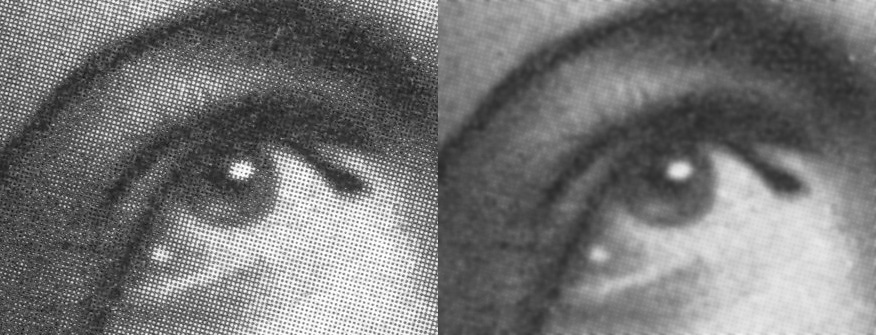
\includegraphics[width=11cm]{Bilder/Gaussian_Blur} \\
 \caption{Anwendung eines Weichzeichnungsfilters}
 \source{https://de.wikipedia.org/wiki/Datei:Halftone,_Gaussian_Blur.jpg}{10.3.2019}
 \label{fig:Blur}
\end{figure}

\subsection{Laplace-Filter}
Ein Laplace-Filter ist ein Faltungskern zur Kantendetektion innerhalb eines Bildes.
Unter einer Kante versteht man hierbei eine rasche Veränderung der Helligkeitswerte entlang einer Richtung.

Um Kanten zu finden wird ein Operator auf das Bild angewendet, welcher die zweite Ableitung bildet (Laplace-Operator). Abrupte Schwankungen der Intensitätswerte werden dadurch als Nulldurchgänge sichtbar.

Über die Faltung des Operators der Vorwärtsdiffenz {\em (1 -1)} mit sich selbst, lässt sich ein 1-dimensionaler Faltungskern der zweiten Ableitung bilden: {\em (1 -2 1)}.
Dieser Kern lässt sich transponieren, um ein Bild nicht nur in x-, sondern auch in y-Richtung abzuleiten.
Beide Kerne kombiniert ergeben den Laplace-Filter:

$$ \left( \begin{array}{rrr}
0 & 1 & 0 \\
1 & -4 & 1 \\
0 & 1 & 0 \\
\end{array}\right) $$

Wendet man diesen Filter auf ein Bild an, erhält man folgendes Ergebnis:

\begin{figure}[ht]
   \centering
     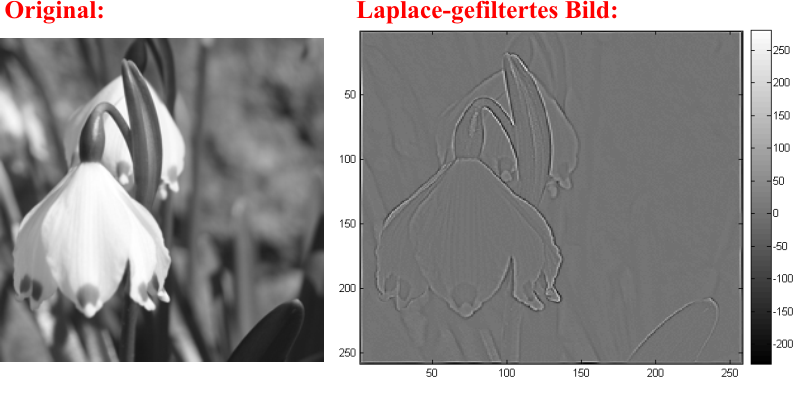
\includegraphics[width=11cm]{Bilder/Laplace} \\
 \caption{Anwendung eines Laplace-Filters}
 \source{https://de.wikipedia.org/wiki/Datei:Laplace_beispiel.png}{10.3.2019}
 \label{fig:Laplace}
\end{figure}

Aufgrund eines hohen Rauschanteils in natürlichen Bildern liefert dieser Filter jedoch nicht immer gute Resultate.

\subsection{Sobel-Operator}
Um auf natürlichen Bildern Kanten zuverlässig zu erkennen, kombiniert der Sobel-Operator die Ideen des Gauß- und Laplace-Filters.
Hierbei wird das Bild in eine Richtung über die zentrale Differenz {\em (1 0 -1)} abgeleitet, andere Richtung jedoch über einen Gauß-Filter {\em (1 2 1)} geglättet,
um Rauschanteile zu reduzieren.
Kombiniert man beide Filter miteinander, erhält man den Sobel-Operator

$$ \left( \begin{array}{rrr}
-1 & 0 & 1 \\
-2 & 0 & 2 \\
-1 & 0 & 1 \\
\end{array}\right) $$

Dadurch werden Kanten jedoch nur in eine Richtung erkannt.
Um Kanten in die jeweils andere Richtung zu erkennen, kann die Faltungsmatrix transponiert werden und ebenfalls auf
das Ausgangsbild angewendet werden.

Die beiden erhaltenen Ergebnisse können nun vereint werden, um alle Kanten innerhalb eines Bildes zu erhalten:

\begin{figure}[ht]
   \centering
     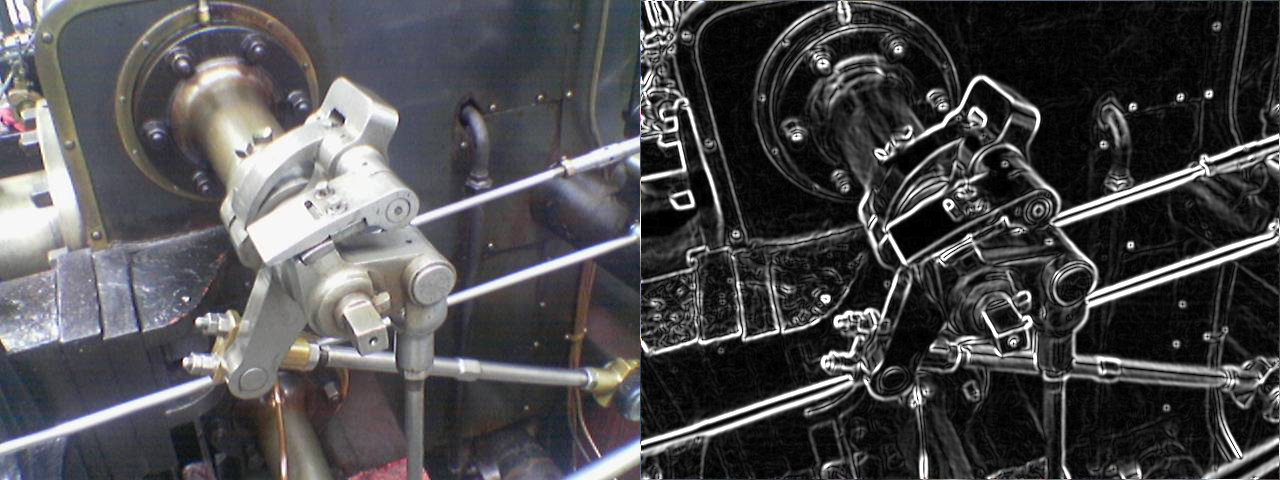
\includegraphics[width=11cm]{Bilder/Sobel} \\
 \caption{Anwendung eines Sobel-Operators}
 \source{https://en.wikipedia.org/wiki/File:Valve_sobel_(3).PNG}{10.3.2019}
 \label{fig:Sobel}
\end{figure}

\section{Canny-Edge-Detection} % Mi
\section{Otsu} % Mi
\section{Haar-Features} % Mi

\section{Morphologische Operatoren} % Mo
\subsection{Erosion}
\subsection{Dilatation}
\subsection{Closing}
\subsection{Opening}

\section{OpenCV} % Mi

\chapter{Analyse}
In diesem Kapitel wird die Problemlage im Bezug zum derzeitigen Stand der Technik analysiert.
Etablierte Verfahren, welche für eine Lösung geeignet wären, werden mithilfe von Bespielen aus der Literatur vorgestellt.
Anschließend werden die Verfahren mit einem geeigneten Testdatensatz evaluiert.
Hierbei werden auch die jeweilige Ressourcenlast und Effizienz gemessen.
Das geeignetste Verfahren wird für den weiteren Verlauf der Arbeit bestimmt.

\section{Stand der Technik}
Bildverarbeitung ist ein Thema, dass schon sehr lange im Bereich der Informationstechnik und Informatik erforscht wird.
Besonders durch derzeitige Entwicklungen in der künstlichen Intelligenz und der Objekterkennung bekommt das Thema in der heutigen Zeit eine hohe Bedeutung für die technische Entwicklung. Im folgenden Kapitel werden einige der zum derzeitigen Zeitpunkt etablierten Verfahren der Bildverarbeitung im Kontext der Aufgabenstellung evaluiert und bewertet.

\subsection{Statische Verfahren}
Verfahren, welche ohne einen speziellen Kontext direkt auf die Pixelwerte eines Bildes angewendet werden können, werden im folgenden als "`statische Verfahren"' beschrieben. 

Diese Verfahren benötigen keine Vorverarbeitung oder Trainingsdaten um verwendet zu werden.
In den meisten Fällen sind diese Verfahren besonders ressourceneffizient, da sie mit weniger Speicher- und Zeitkomplexität auskommen.
\subsubsection{Pixelorientierte Bildanalyse}
\textbf{Beschreibung}\newline
Ein trivialer Ansatz um Veränderungen zwischen zwei oder mehreren Bildern zu erkennen kann durch einen Vergleich der Pixelwerte ermöglicht werden.
So ist es auch möglich benachbarte Pixel in einem Bild nach bestimmten Veränderungen abzusuchen.
Bei den möglichen Veränderungen handelt es sich dabei um statistisch messbare Merkmale wie unter anderem auch Intensität, also Helligkeit, sowie die jeweiligen Farbwerte.

Helligkeits- oder Farbwechsel können im Bezug zur Objekterkennung auf einem Bild verwendet werden, indem man zum Beispiel eine Reihe an sogenannten "`Hintergrund"'-Pixeln wählt und diese mit den benachbarten Objektpixeln vergleicht.
Für den Fall der Verkehrskameras würde der besagte Hintergrund die Pixelwerte der Straße in dem gewählten Bereich beschreiben.
Sobald eine Reihe von Pixeln durch einen starken Farb- oder Intensitätswertwechsel unterbrochen wird, kann man in diesem Fall von einem beweglichen Objekt auf der Straße ausgehen.\newline\newline
\textbf{Literatur}\newline
O.K. Rahmat und Jumari beschreiben in ihrer Arbeit~\cite{bin2001vehicle} ein solches Verfahren und wenden dies auf Bilder von Verkehrskameras an. 
Die Besonderheit ist hierbei, dass nicht alle Pixelwerte des Bildes verglichen werden, sondern nur ein relevanter Teilabschnitt zu Vergleichszwecken ausgesucht wird. 
Dieser Teilbereich wird von den Autoren auch als "`Detektor"' beschrieben und befindet sich in der Mitte einer ausgewählten Fahrbahn. 
So werden auf Straßen mit mehreren Fahrbahnen auch mehrere solcher Detektoren benötigt.

Ziel ist es, wie bereits beschrieben die Intensität in dem Bereich eines Bildes zu überwachen. 
Sobald es einen stark abweichenden Wert gibt, wird davon ausgegangen das ein Auto den Streckenabschnitt des Detektors durchfährt und ein Zähler wird inkrementiert.
Die Länge eines stockenden Verkehrsflusses kann ebenfalls über diese Methode ermittelt werden. 
Hierfür wird in der Arbeit der beiden Autoren ein länglicher Detektor verwendet der sich über den kompletten im Bild ersichtlichen Streckenabschnitt zieht.
Weiterhin werden die Farbwechsel innerhalb der Detektoren ausgewertet, um die einzelnen Objekte voneinander zu trennen.
\newline\newline
\textbf{Fazit}\newline
Das Verfahren hat eine sehr geringe Komplexität und ist daher einfach zu implementieren, jedoch werden auch schon in der Arbeit Situationen beschrieben in denen das Verfahren keine zuverlässigen Ergebnisse liefert. 
So kann zum Beispiel der Lichtkegel eines Scheinwerfers bei Nacht das Ergebnis verfälschen.
\begin{figure}[ht]
   \centering
     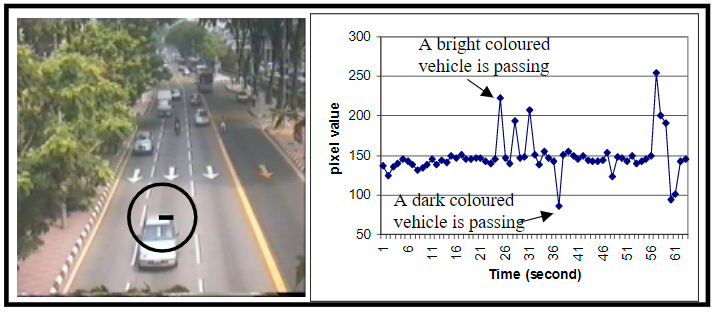
\includegraphics[width=15cm]{Bilder/pixelanalysis} \\
 \caption{Detektor im Einsatz}
 \sourceref{bin2001vehicle}
 \label{fig:Pixelanalysis}
\end{figure}
\newpage
\subsubsection{Kantenerkennung}
\textbf{Beschreibung}\newline
Kantenerkennung bezeichnet eine Klasse von Verfahren, bei welchen Kanten im Bild über abrupte Intensitätswert-Übergänge gefunden werden. 
Dabei werden in der Regel Faltungskerne (siehe \ref{sec:Faltungskerne}) verwendet, um die Ableitung der Intensitätswert-Funktion in einem Grauwert-Bild zu ermitteln.

Das bedeutet für die Anwendung des Verfahrens muss das Bild in den Grauwert-Bereich übertragen werden.
Die entstandenen Kanten (Abbildung~\ref{fig:gupte1}) können dann anschließend für die Objekterkennung verwendet werden. 
Um leicht überlagernde Objektkanten voneinander zu trennen können morphologische Operatoren verwendet werden (siehe \ref{sec:MorphologischeOperatoren}).
Diese werden auch verwendet um kleine irrelevante Kanten aus dem Bild zu entfernen.
\newline\newline
\textbf{Literatur}\newline
Gupte und Papanikolopoulos stellen eine exemplarische Implementierung  des Verfahrens in ihrer Arbeit~\cite{gupte2000algorithms} vor. 
Dabei werden Kanten auf zwei Bildern einer Verkehrskamera erkannt und dann beide Kantenbilder per XOR vereinigt. 
Dies ermöglicht das erkennen von Veränderungen zwischen den beiden Bildern der Verkehrskamera.
Mögliche Veränderungen können in diesem Fall auf ein bewegliches Objekt, wie zum Beispiel ein Auto, hindeuten.

Das Ergebnis wird anschließend mithilfe von der Anwendung von mehreren Dilatation-Operationen verbessert, da nicht geschlossene und im Objekt liegende Kanten zur einer großen Kante verbunden werden (Abbildung~\ref{fig:gupte2}).
Für den Fall das nach der Anwendung der jeweiligen Operationen immer noch unverbundene Kanten vorliegen werden nah benachbarte Kanten durch ein großes Rechteck umkreist.
Das resultierende Rechteck ist in diesem Fall dann das erkannte Objekt.
\newline\newline
\textbf{Fazit}\newline
Dieses Verfahren ist ebenfalls wenig komplex und lässt sich einfach implementieren. 
Jedoch besitzt es auch einige Nachteile, wie zum Beispiel, dass sich Schattenwurf negativ auf das Ergebnis auswirkt und eine Perspektive im Bild vorausgesetzt wird.
Wettereinflüsse wie Regen oder Schnee würden sich ebenfalls sehr negativ auf das Ergebnis auswirken.
Es existieren viele Implementierungen des Verfahrens, wobei die Arbeit von Gupte und Papanikolopoulos nur ein Beispiel ist.
So lassen sich auch durch Vorverarbeitung oder Maskierung der Bilder möglicherweise das Ergebnis verbessern.

\begin{figure}[ht]
  \centering
	\begin{minipage}[b]{0.4\textwidth}
     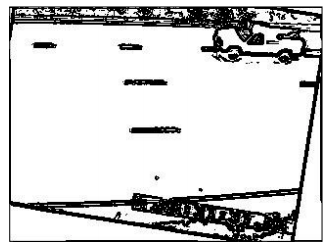
\includegraphics[width=\textwidth]{Bilder/gupte1} \\
   \caption{Kantenerkennung}
	 \sourceref{gupte2000algorithms}
   \label{fig:gupte1}
  \end{minipage}
	\hfill
	\begin{minipage}[b]{0.4\textwidth}
     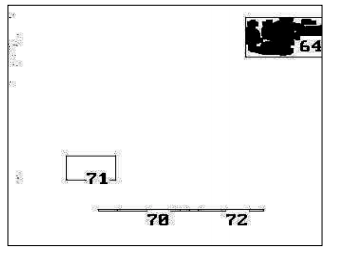
\includegraphics[width=\textwidth]{Bilder/gupte2} \\
		\caption{Ergebnis des~\newline Verfahrens}
	 \sourceref{gupte2000algorithms}
		\label{fig:gupte2}
	\end{minipage}
\end{figure}
\newpage

\subsection{Dynamische Verfahren}
Als "`dynamische Verfahren"' werden im folgenden Verfahren beschrieben, die nur innerhalb eines bestimmten Kontextes auf ein Bild angewendet werden sein. So kann es sein, dass das Verfahren bestimmte Trainingsdaten oder Vergleichswerte von anderen Bildern benötigt. Dies erhöht in den meisten Fällen die Genauigkeit des Verfahrens, aber die Ressourceneffizienz wird drastisch verringert.
\subsubsection{Neuronale Netze}
\textbf{Beschreibung}\newline
Neuronale Netze sind ein Beispiel für Verfahren aus dem maschinellen Lernen.
Hierbei wird versucht die Arbeitsweise des menschlichen Gehirns nachzuempfinden.
Neuronale Netze besitzen daher auch eine Art internen Speicher der antrainiertes Wissen abbildet.
Ein neuronales Netz kann somit für eine bestimmte Aufgabe trainiert werden, welche dann relativ zuverlässig von dem Netz gelöst werden kann.
Ziel von dem Training ist hierbei durch Anwendung des Netzes die Fehlerquote zu minimieren.
Sobald ein neuronales Netz fertig trainiert wurde kann der Zustand des Netzes serialisiert und abgespeichert werden, damit es in der Zukunft weiterverwendet werden kann.
\newline\newline
\textbf{Literatur}\newline
In der Arbeit \cite{hkkDhbw} wurden sogenannte "`konvolutionale"' neuronale Netze für die Erkennung von stockendem Verkehr auf Bildern verwendet (siehe Abbildung~\ref{fig:CNN}).
Diese Netze nutzen unter anderem auch Faltungskerne (siehe~\ref{sec:Faltungskerne}) um Objektklassifizierung auf einem Bild durchzuführen.

Diverse Schichten von Neuronen werden in einem der verwendeten neuronalen Netze verwendet, um die aus den Pixelwerten gewonnenen Informationen auf eine konkrete Einschätzung bezüglich des Verkehrsflusses herunterzubrechen.
So kann eine Pixelmatrix als Eingabe an das neuronale Netzwerk weitergegeben werden und als Ausgabe ein einfacher boolescher Wert (eins oder null) empfangen werden. 
Eine Eins wäre beispielsweise eine positive Rückmeldung dafür dass auf dem Bild stockender Verkehr sichtbar ist.

Wichtig hierbei sind die einzelnen Verbindungen zwischen den Neuronen-Schichten, welche je nach Training und Zustand des Netzes unterschiedlich gewichtet werden.
\begin{figure}[ht]
   \centering
     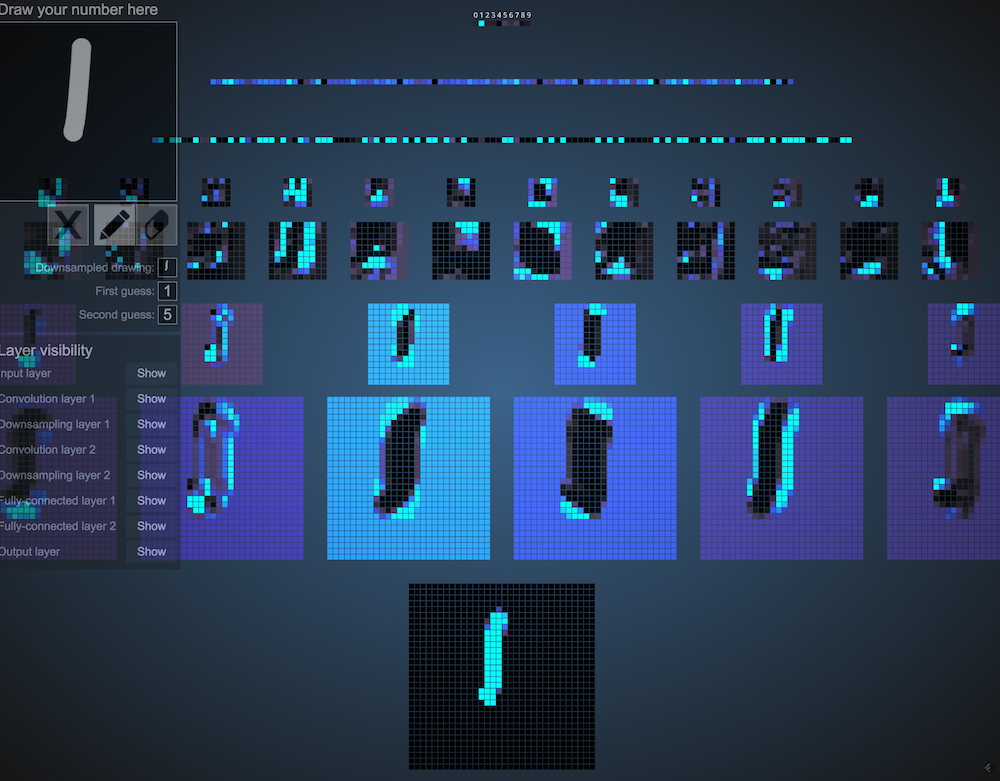
\includegraphics[width=15cm]{Bilder/cnn-visualized} \\
 \caption{Visualisierung der Schichten eines konvolutionalen neuronalen Netzwerks (unten Eingang - oben Ausgabe)}
 \source{http://scs.ryerson.ca/~aharley/vis/}{12.4.2019}
 \label{fig:CNN}
\end{figure}
\newline\newline
\textbf{Fazit}\newline
Bei der Laufzeit eines komplexen neuronalen fällt Netzes auf, dass das Laden und Benutzen der Neuronen einen relativ hohen Hauptspeicher-Bedarf mit sich bringt.
Der Vorteil der sich jedoch hierdurch bietet ist, dass Bilder nicht statisch analysiert werden, sondern das Netz dynamisch auf Bilder und Verhältnisse, wie zum Beispiel Perspektive und Wetter, trainiert wird.
Dieses Verfahren wurde für die folgende Implementierung nicht gewählt, da diese Arbeit einen besonderen Fokus auf die Ressourcensparsamkeit des Verfahrens setzt.
\newpage

\subsubsection{Background Subtraction}
\textbf{Beschreibung}\newline
Background Subtraction, auch als Foreground Detection bekannt, ist eine Klasse von Verfahren, bei denen einer Serie von Bildern auf Veränderungen analysiert wird.
Ziel ist es sich bewegende Objekte im Vordergrund des Bildes vom Hintergrund zu trennen.
Hierfür wird ein sogenanntes Hintergrund-Modell aus den ersten Bilder der Serie generiert, welches dann auf das letzte Bild angewandt wird, um ein Objekt im Vordergrund zu erkennen. 
Diese verwenden Statistiken, welche über alle Bilder der Serie generiert werden, um Gemeinsamkeiten zwischen den Bildern zu erkennen.

In dem Artikel \cite{mcivor2000background} werden mehrere dieser Hintergrund-Modelle im Detail beschrieben.
Bei der Auswahl des geeigneten Hintergrund-Modells sind mehrere Parameter zu berücksichtigen, wie zum Beispiel Perspektive und Farb- und Intensitäts-Spektrum.
\newline\newline
\textbf{Literatur}\newline
Akoum beschreibt im Artikel \cite{akoumBSIP} wie das Hintergrund-Modell "`Gaussian mixture Models"', oft auch als "`Mixtures of Gaussians"' beschrieben, auf ein Video einer Verkehrskamera angewandt werden kann.
Bei diesem Hintergrund-Modell werden alle Intensitätswerte der Pixel eines Bildes mithilfe eines Gaußschen Mischmodells modelliert.

Ein Gaußsches Mischmodell ist dabei ein statistisches Clusterverfahren, welches die Hintergrundpixel kategorisiert.
Alle Pixel die nicht über das Mischmodell kategorisiert werden konnten sind somit Vordergrund-Pixel und somit auch mögliche Objekte im Vordergrund.
Objekte die im Bild durch das Verfahren erkannt wurden sind im Anschluss weiß eingefärbt, während der Hintergrund schwarz eingefärbt wird.
Das Ergebnis des Verfahrens wird mit Dilatations- und Erosions-Filtern im Anschluss verbessert. 
Der Dilatations-Filter sorgt dabei für die Verbindung von nicht geschlossenen Kanten, während der Erosions-Filter kleine unwichtige Kanten aus dem Bild entfernt.
\newline\newline
\textbf{Fazit}\newline
Das Verfahren ist relativ komplex, bietet dafür aber eine sehr gute Genauigkeit. 
Aufgrund des Hintergrund-Modells müssen jedoch mehrere sich unterscheidende Bilder für das Verfahren verwendet werden.
Im Falle der Verkehrsanalyse sollte dies kein Problem darstellen, da eine fixierte Kamera bereits gegeben ist, welche jede Minute ein neues Bild aufnimmt.
Parameter die für das anwenden des Hintergrund-Modells benötigt werden müssen im Hauptspeicher vorbehalten werden.
Daher hat dieses Verfahren auch nicht die beste Speichereffizienz.
Dennoch können durch die jeweiligen Hintergrund-Modelle auch Wetter- und Lichtveränderungen miteinbezogen werden, was potentielle Fehlerquellen in den statischen Verfahren waren.
Weiterhin gibt es bereits einige Implementierungen diverser Hintergrund-Modelle in der Bibliothek OpenCV (siehe \ref{sec:OpenCV}).
\begin{figure}[!ht]
   \centering
     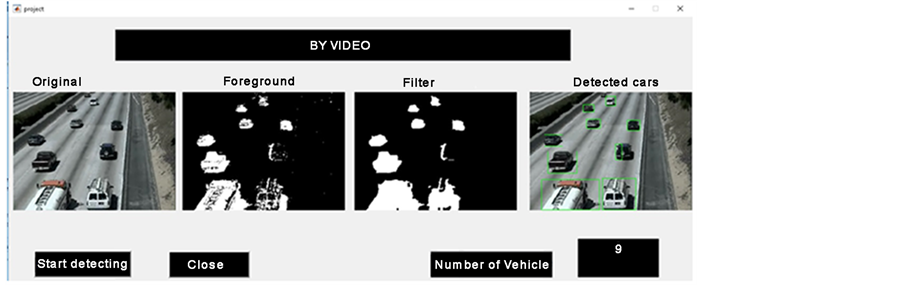
\includegraphics[width=15cm]{Bilder/mogpaper} \\
 \caption{Background Subtraction im Einsatz}
 \sourceref{akoumBSIP}
 \label{fig:BSSoftware}
\end{figure}
\newpage

\section{Bestimmung des Testdatensatzes}
\subsection{Verkehrskameras laden}
\label{sec:AnaCam}
Bevor die Kamerabilder geladen werden können, ist es zunächst relevant zu wissen welche Kameras es überhaupt gibt und wo diese liegen.
Hierfür stellt die Verkehrszentrale eine Liste aller Kameras unter dieser Webadresse bereit: \url{http://www.svz-bw.de/kamera/kamera_A.txt} (Stand: 31.3.2019).

Diese liegen in einer durch Tabulatorzeichen separierten Tabellenstruktur vor.

\begin{center}
\scriptsize
    \begin{tabular}{ | l | l | l | l | l | l | l | l |}
    \hline
		lon & lat & title & description & linkextern & icon & iconSize & iconOffset \\ \hline
    572330.13 &
		5361095.33 &
		... &
		/.../kameradetail.php?id=EXT006 &
		... &
		... &
		16,16 &
		-8,-8 \\
    \hline
    \end{tabular}
\end{center}

Die Werte {\em lat} und {\em lon} beschreiben die Position der Kamera durch Längen und Breitengrad.
Der Eintrag {\em title} enthält einen ausfühlicheren Titel der Kamera. Mit {\em description} hat man die Möglichkeit eine detailiertere Beschreibung der Kamera zu erhalten, welche jedoch mit HTML Tags angereichert ist. {\em Linkextern} ist die Webadresse, über welche auf die Kamera zugegriffen werden kann. {\em Icon}, {\em iconSize} und {\em iconOffset} sind Informationen, die das Straßenverkehrszentrum selbst benötigt, um das Kameraicon auf einer Landkarte anzuzeigen.

Relevant sind also zunächst die Koordinaten, der Titel und der Link, da nur über diesen die ID der Kamera aufgelöst werden kann.
Das erste Problem hierbei ist, dass die Koordinaten der Kamera nicht der üblichen Projektion der Weltkugel entsprechen. Gebräuchlich ist die Projektion {\em WGS 84}~\cite{wgs84}, welche auch von Navigationssystemen oder herkömlichen Kartendiensten genutzt wird und den Globus von -180° westlich bis 180° nördlich, bzw. -90° südlich bis 90° nördlich einteilt.

Das Straßenverkehrszentrum nutzt jedoch das Referenzsystem {\em ETRS89 / UTM zone 32N}~\cite{etrs89}, welches für Europa ausgelegt ist.
Um Position der Kameras mit gängigen Kartendiensten nutzen zu können müssen die Koordinaten in die übliche Projektionsform überführt werden.

Außerdem muss die ID der Kamera aus dem Link extrahiert werden, da es keinen Eintrag in der Tabelle gibt, der lediglich die ID enthält.
Da die Link immer dem selben Format folgt ({\em /<pfad>/kameradetail.php?id=<id>}), kann einfach nach dem Vorkommen der Teilzeichenkette {\em ?id=} gesucht werden, und alles davor abgeschnitten werden.

Somit lassen sich alle relevanten Informationen, welche für die Weiterverarbeitung der Kameras benötigt werden, abrufen.

\subsection{Verkehrsbilder laden}
Sobald die ID einer Kamera verfügbar ist, lassen sich auch die Kamerabilder abrufen.
Die Bilder werden im Regelfall alle 1-5 Minuten aktualisiert und im JPEG Format auf dem Server der Straßenverkehrszentrale öffentlich gemacht.
Es sind daher keine Videosequenzen, sondern nur Einzelbilder verfügbar.

Über die URL {\em https://www.svz-bw.de/kamera/ftpdata/<id>/<id>\_gross.jpg} lässt sich stets die aktuellste Aufnahme für eine Kamera abrufen, wobei {\em <id>} der ID der Kamera entsprechen muss.

Jedoch verbietet die Straßenverkehrszentrale den Zugriff auf die Bilder von außerhalb ihrer Webpräsenz.
Um dennoch darauf zugreifen zu können, kann der {\em Referer} HTTP-Header mit dem Hostnamen der Verkehrszentrale (http://svz-bw.de) beim Abrufen des Bildes mitgesendet werden, wodurch der Zugriff gewährt wird. 

\subsection{Vergleichsdatensätze generieren}
Bevor verschiedene Verfahren getestet und miteinander verglichen werden können, wird zunächst ein Vergleichsdatensatz benötigt.

%Hierzu reicht es jedoch nicht einfach Bilder herunterzuladen und diese selbst zu klassifizieren, denn manche Verfahren müssen zunächst trainiert werden. Background-Subtraction benötigt beispielsweise 5-10 Bilder als Training, um Hintergrund von Vordergrund unterscheiden zu können.

%Es muss also immer eine Gruppe von zeitlich nahe beieinanderliegenden Bildern vorliegen, um diese Auswerten zu können.

Um nun den Datensatz zu generieren wird ein Python-Skript verwendet.
Wird dieses gestartet, fängt es an periodisch für einige der Kameras auf der A5 Bilder herunterzuladen.

Neben den Bildern selbst wird auch eine Metadatei im JSON-Format generiert.
Diese enthält zunächst einen Zeitstempel, wann das Bild erstellt wurde.
Außerdem enthält diese auch noch, wie viele Autos jeweils auf der linken und rechten Spur zu sehen sind, und ob anhand dessen Stau ist oder nicht.

Um diese Informationen zu generieren, wird ein sehr prototypischer Algorithmus verwendet. Die Resultate sind dementsprechend nicht gerade akkurat, weshalb ein Mensch diese zusätzlich verifizieren muss. Um jedoch den Menschen dabei zu unterstützen, ist eine grobe Vorauswertung sehr Hilfreich.

Um als Mensch die Bilder auswerten zu können, kann ein zweites Skript Abhilfe schaffen.

Dazu gibt es in den Metadaten ein Feld, welches speichert, ob ein Bild bereits von einem Menschen verifiziert wurde.
Mit dem Skript werden nun nacheinander alle noch nicht ausgewerteten Bilder angezeigt, wobei abwechselnd die linke, bzw. rechte Spur maskiert werden. Zusätzlich sieht man, ob die Vorauswertung für die angezeigte Spur Stau erkannt hat, oder nicht.

Als Mensch hat man nun die Möglichkeit durch das Drücken der Enter-Taste zu speichern, dass Stau auf dem Bild zu sehen ist, bzw. durch das Drücken einer anderen Taste zu bestätigen, dass kein Stau zu sehen ist.

Anschließend wird das nächste Bild, bzw. die nächste Spur angezeigt.
Dies passiert solange, bis keine Bilder mehr ausgewertet werden müssen, bzw. der Nutzer das Skript beendet.

\section{Auswahl des Verfahrens}
Zur Auswahl des bestmöglichen Verfahrens werden verschiedene Ansätze anhand des Testdatensatzes ausgewertet.

\subsection{Helligkeit}
Das erste Verfahren Klassifiziert ein Bild lediglich anhand der Häufigkeit der Intensitätswerte.
Dazu werden zunächst, wie beim Histogramm, die Intensitätswerte zwischen 0 und 255 aufsummiert.
Anhand eines Schwellwertes, in unserem Fall der Grauwert 40, wird dann versucht das Bild zu klassifizieren.
Gibt es in Summe mehr Grauwerte unter dem Schwellwert, als darüber, wird Stau auf dem Bild angenommen.
Die Überlegung dahinter ist, dass die Straße einen sehr neutralen bis hellen Grauton aufweist. Fahren nun Autos auf der Fahrbahn, dann können diese in verschiedensten Farben, sowohl über, als auch unter dem Schwellwert auftreten.
Jedoch werden von den Autos auch Schatten geworfen, welche die Straße verdunkeln, und so die Intensitätswerte reduzieren.
	
\subsection{Haar-Features}
Der Ansatz zur Stauerkennung über Haar-Features verläuft etwas anders als die Erkennung über die Helligkeit.
Hierbei wird versucht über Autos zu klassifizieren, um diese anschließend zu zählen und abzuschätzen, ob Stau ist, oder nicht.

Zur Klassifizierung der Autos kann ein von OpenCV mitgelieferter Cascade-Classifier zur Erkennung von Autos genutzt werden.
Dieser ist standardmäßig bei OpenCV verfügbar und soll über Haar-Features Autos auf Bildern erkennen können.
Solche Kaskaden werden als XML-Dateien mitgeliefert, welche über die Methode {\em CascadeClassifier} geladen werden können.

Anschließend kann damit ein Bild untersucht werden. Als Ergebnis erhält man eine Liste von Konturen, welche Autos auf dem Bild darstellen sollen.

% TODO: Insert image

Die Ergebnisse dieses Verfahrens sind jedoch nicht so gut, da die Auflösung der Kameras zu gering sind, sodass die Merkmale von Autos nicht deutlich genug sind, um diese als Autos klassifizieren zu können.
Besser arbeiten Classifier auf Bild-Sequenzen, wie z.B. Videos, da diese dabei helfen Autos über die Sequenzen hinweg zu verfolgen.
Da die Straßenverkehrszentrale jedoch nur Einzelbilder liefert, sind die Ergebnisse nicht sehr genau.

\subsection{Edge detection}
* Erkennen der Kanten über Canny\newline
* Anhand der Kanten Bild Segmentieren und Konturen herausarbeiten zur Erkennung von Merkmalen und Klassifikation\newline
* Auflösung der Kamerabilder zu gering und Bilder recht unscharf mit viel zu Rauschen\newline
* Zu viele Kanten werden erkannt, um Autos verlässlich erkennen zu können\newline
* Mittelung des Bildes über Gauß zeigt keine signifikante Verbesserung aufgrund der zu niedrigen Qualität\newline
	
\subsection{Background Subtraction}
* Viele Bilder über möglichst kurzen Zeitabstand aufsummieren\newline
* Anhanddessen Hintegrund errechnen\newline
* Hintegrund vom Zielbild abziehen\newline
* Übrig bleiben nur noch Autos\newline
* Morphologische Operatoren zur Nachoptimierung\newline
* Konturen zählen -> Anzahl der Autos\newline
* Über Anzahl der Autos Rückschlüsse über Verkehrssituation ziehen\newline
* Verschiedene BGS algorithmen in OpenCV verfügbar (GSOC, KNN, CNT, GMG, LSBP, MOG, MOG2)\newline
* MOG liefert beste Ergebnisse für konkretes Einsatzgebiet\newline
* Jedoch mehrere Bilder nötig, um Hintergrund verlässlich zu erkennen\newline
* Bei absolutem Stau (keine Bewegung der Autos über längere Zeit ~10min) keine Erkennung des Hintergrundes möglich\newline

\subsection{Auswahl}
* BGS is top

\chapter{Implementierung}
Im folgenden Kapitel wird die praktische Implementierung der in der Arbeit erarbeiteten Methode beschrieben. Die Implementierung umfasst dabei die Schnittstelle zum Nutzer, sowie die Erhebung, Verarbeitung und Persistenz von relevanten Daten.
\section{Backend}
Für die Implementierung der Arbeit wurde ein Backend konzipiert, welches Informationen und Bilder von Verkehrskameras für Clients vorenthält. Das Ziel ist es dabei Daten der Straßenverkehrszentrale regelmäßig anzufragen und für den Client zu persistieren. Somit wird ermöglicht, dass der Client auch auf ältere Datensätze der Straßenverkehrszentrale zugreifen kann. Weiterhin ermöglicht soll das Backend die Daten in einem möglichst kompakten Format an den Client senden können, damit auch über schwache zelluläre Netzwerkverbindungen von Clients die Daten relativ zügig empfangen können. 
\subsection{Infrastruktur}
Im Rahmen der Implementierung des Backends wurden diverse Anforderungen an die zu verwendenden Technologien beachtet. So soll die resultierende Anwendung auf dem Apache Server eines geteilten Webhosts laufen. Der Apache Server des Webhosts erlaubt das Ausführen von PHP-Skripten, welche für Anfragen und Verarbeitung von Daten der Straßenverkehrszentrale Baden-Württemberg verwendet werden können. Für die Persistenz von Daten besitzt der Webhost alternativ zum Dateisystem auch eine MySQL-Datenbank.
\begin{figure}[hp]
   \centering
     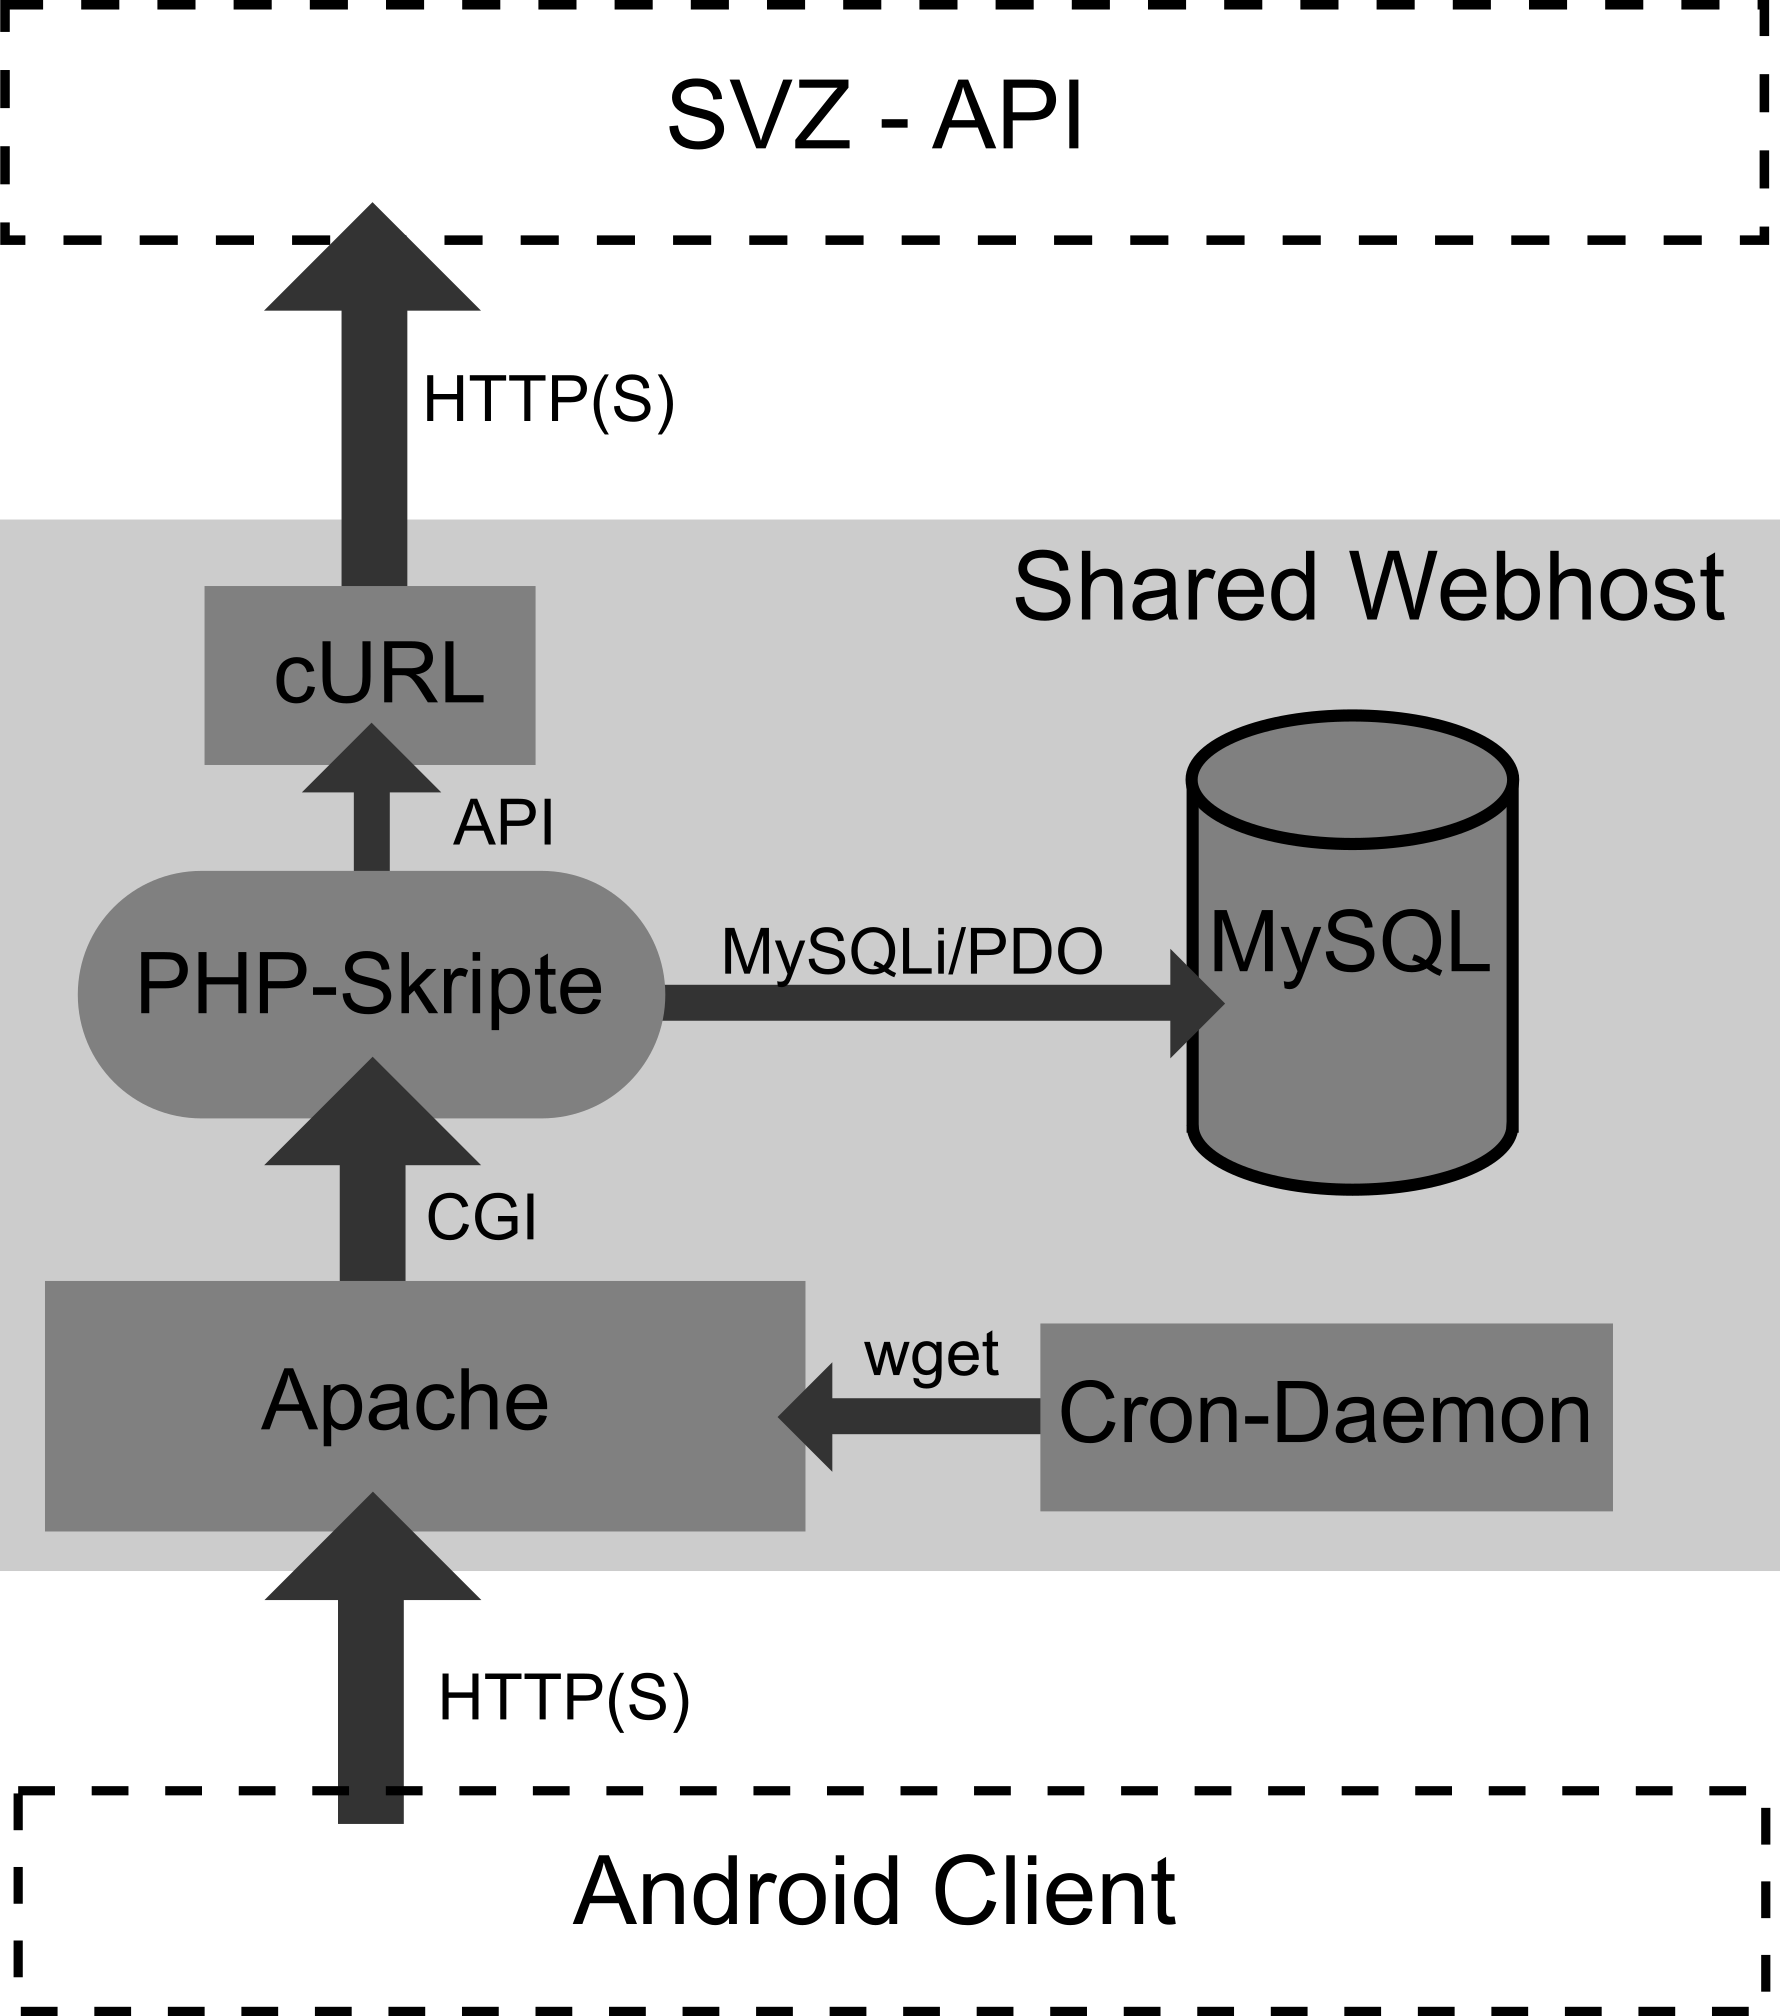
\includegraphics[width=13cm]{Bilder/server-arch} \\
 \caption{Server Architektur}
 \label{fig:serverarch}
\end{figure}

Auf Abbildung~\ref{fig:serverarch} ist zu sehen, dass die Verbindung zum Client über das HTTP-Protokoll verläuft. Der Vorteil ist hierbei, dass das Protokoll bereits von dem Apache Server unterstützt wird und eine Verschlüsselung über TLS eingesetzt werden kann.
\subsection{Datenerhebung}
\label{sec:datenerhebung}
Die Erhebung von benötigten Daten erfolgt durch HTTP-Anfragen an den Server der Straßenverkehrszentrale. Diese können mithilfe der cURL-API in PHP angestoßen werden. Bei "`cURL"' handelt es sich dabei um eine Programm-Bibliothek, mithilfe welcher sich Daten über verschiedene Protokolle übertragen lassen.

Informationen über die jeweiligen Kameras werden über den SVZ-Server in verschieden Formaten bereitgestellt. So sind die Metadaten der Kameras als Textdatei abgespeichert, während die Bilder direkt im JPEG-Format abgerufen werden können. Unter Metadaten der Verkehrskameras sind bei folgende Informationen zu verstehen: 
\begin{itemize}
\item{Eine eindeutige alphanumerische Kamerakennung}
\item{Die entsprechende Autobahnkennung}
\item{Name der nächsten Ausfahrt mit Autobahnkennung}
\item{Position der Kamera}
\end{itemize}
Die Metadaten der Kameras müssen nur einmalig abgerufen und verarbeitet werden, während die Bilder der Verkehrskameras von der SVZ alle 30 Sekunden erneuert werden. 
Um immer aktuelle Datensätze zu empfangen werden Bilder im 30-Sekunden-Takt angefragt. Dies lässt sich über PHP und einen Cronjob im Linux Betriebssystem des geteilten Webhosts realisieren.
Ein Datensatz der nicht über HTTP-Aufrufe erhoben werden kann sind Masken für Bilder einer Verkehrskameras.
Dabei handelt es sich um Bilder im PNG-Format, welche zur Vorverarbeitung von Bildern verwendet wird. Diese müssen manuell erstellt und in die Datenbank eingepflegt werden, da im Rahmen der Arbeit kein vollständig korrekter Algorithmus zur Automatisierung dieser Aufgabe gefunden wurde.

\subsection{Datenpersistenz}
Für die Persistenz von Daten wurde während der Implementierung auf das Dateisystem verzichtet und nur die MySQL-Datenbank verwendet, da diese die Vorteile einer relationalen Datenbank, sowie sichere Transaktionen bietet.
Bei den Datensätzen die zu persistieren sind handelt es sich dabei um:
\begin{itemize}
\item{Die Metadaten einer Verkehrskamera (siehe \ref{sec:datenerhebung})}
\item{Die Bilder einer Kamera im JPEG-Format}
\item{Die Masken für eine Kamera im PNG-Format}
\end{itemize}
Jeder dieser Datensätze besitzt in der Datenbank eine eigene Tabelle mit einem jeweils eigenen Datenbank-Schema. 
Wichtig bei der Erstellung der jeweiligen Schemata war dabei geeignete Datentypen für die Bilder zu finden, damit diese korrekt und vollständig eingepflegt werden können.
Das Schema für die Datenbank ist auf Abbildung~\ref{fig:dbschema} zu sehen (Primärschlüssel ist fett gedruckt). "`ABID"' bezeichnet dabei die jeweilige Kennung für die Straße. Ein Beispiel hierfür wäre die Autobahnkennung A5.
\begin{figure}[ht]
   \centering
     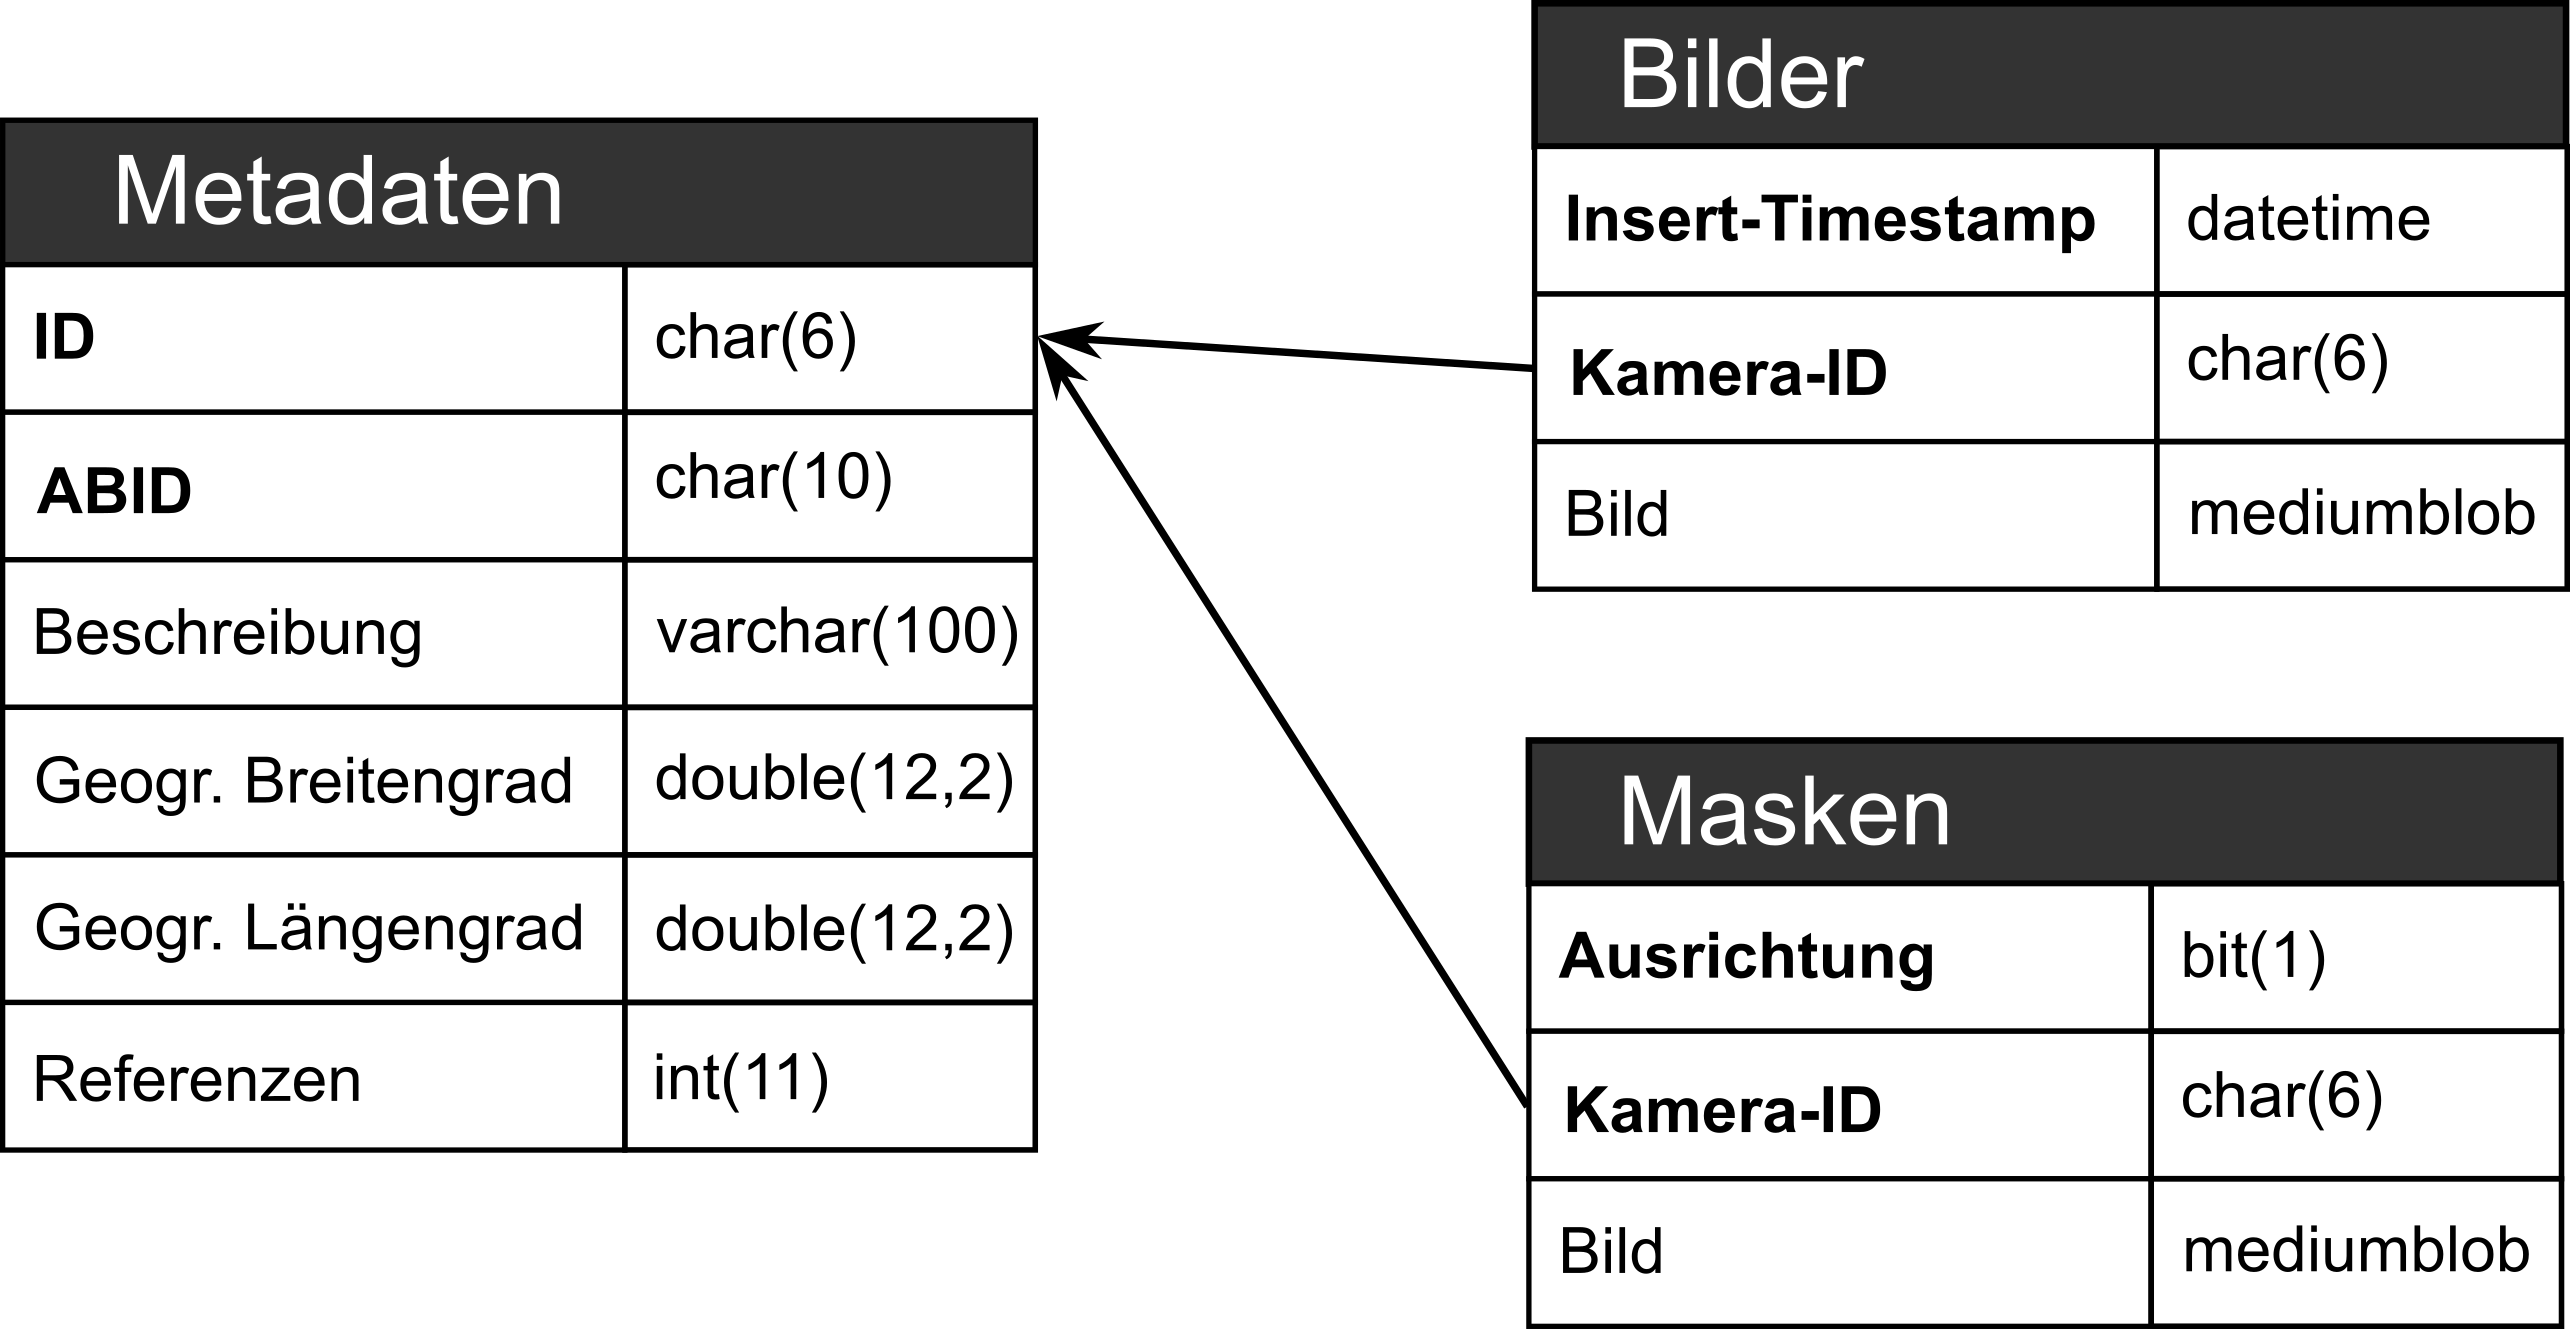
\includegraphics[width=15cm]{Bilder/db-schema} \\
 \caption{Datenbank Schema}
 \label{fig:dbschema}
\end{figure}

Damit PHP-Skripte auf die MySQL-Datenbank zugreifen können gibt es zwei unterschiedliche APIs: Die "`PDO"'-API und die MySQLi-API. 
PDO steht dabei für PHP Data-Objects und bietet eine Unterstützung von mehreren Datenbank-Treibern. 
MySQLi, auch MySQL Improved Extension, begrenzt sich auf die Unterstützung MySQL, bietet aber auch eine erweiterte Unterstützung neuer Funktionen von MySQL.
Da sich die Implementierung in dieser Arbeit auf eine MySQL-Unterstützung beschränkt wurde die letztere Programmier-Schnittstelle verwendet.

Damit die Datenbank mit Bildern, welche alle 30 Sekunden gespeichert werden, vollläuft gibt es einen Lösch-Mechanismus der alte Datensätze automatisch aufräumt. 
Dieser ist in PHP implementiert und überprüft nach dem Einfügen eines Datensatzes, ob mehr als 10 Datensätze vorhanden sind.
Falls dies der Fall ist werden alle Datensätze, welche älter als der zehnt älteste Datensatz sind, gelöscht.

\subsection{Datenbereitstellung}
Daten lassen sich vom Client, wie auf Abbildung~\ref{fig:serverarch} zu sehen, über HTTP-Anfragen an PHP-Skripten abrufen. Es gibt hierbei unterschiedliche Skripte, die für jeweils unterschiedliche Datensätze und Darstellungsarten verantwortlich sind:
\begin{itemize}
\item{kameras.php: Zuständig für das Abrufen aller erreichbaren Kameras mit deren Kennung}
\item{fetchmask.php: Zuständig für die Abfrage einer Maske für eine Verkehrskamera}
\item{fetcher.php: Zuständig für Abfragen von Bildern einer Verkehrskamera}
\end{itemize}
Das Skript "`kameras.php"' gibt bei einer Anfrage eine leerzeichen-separierte Liste aller Kennungen von Kameras zurück, welche eine Maske besitzen und einen Referenzzähler größer eins. 
Der Referenzzähler ist dabei eine Hilfsvariable für das Backend, welche Kameras von Clients benötigt werden und daher die Bilder von ihnen heruntergeladen werden sollten.
Ein Client kann für eine oder mehrere Kameras den Referenzzähler inkrementieren, indem er das "`refcounter.php"' Skript mit den jeweiligen PHP-Skripten aufruft.

Das Skript "`fetchmask.php"' wird mit zwei Query-Paramteren aufgerufen: der Kamerakennung und der Ausrichtung, wobei letzteres ein Binärwert ist. 
Es liefert, wie der Name bereits verrät, das PNG-Bild einer Maske für eine Kamera.

Das letzte Skript "`fetcher.php"' wird mit nur einem Query-Parameter für die Kamerakennung aufgerufen. 
Dieses Skript liefert einen Binärstrom aller gespeicherten Bilder einer Verkehrskamera, sowie den jeweiligen Zeitpunkt (in Unix-Zeit), wann dieses Bild auf dem SVZ-Server gespeichert wurde. 
Damit diese Daten korrekt vom Client gelesen werden können werden die Daten in folgender Reihenfolge gesendet: Die Länge in Bytes des Zeitpunktes und des Bildes zusammen, der Zeitpunkt und Unix-Zeit und abschließend die Bytes des zusendenden JPEG-Bildes.
\newpage

\section{Client}
Der Client wird als eine Android Anwendung realisiert, die durch Kommunikation mit dem Backend und der Straßenverkehrszentrale das Problem der Stauerkennung so effizient und ressourcensparend wie möglich löst.
Durch das Verlagern der Berechnungen auf das mobile Endgerät bleibt die Last des Backends gering und die Rechenleistung des Smartphones wird soweit ausgeschöpft, dass Berechnungen effizient, aber sparsam durchgeführt werden können.

\subsection{OpenCV}
Der Kern der Verarbeitung wird durch Algorithmen der OpenCV Bibliothek~\ref{sec:OpenCV} umgesetzt.
Da OpenCV primär als native Bibliothek zur Verfügung steht, bzw. die für Android nutzbare Java-Schnittstelle auf die native (in C++ geschriebene) Implementierung
zurückgreift, muss OpenCV für die jeweiligen Prozessoren der Android Geräte kompiliert werden, auf denen die Anwendung genutzt werden soll.

Eigentlich bietet OpenCV selbst bereits vorkompilierte Versionen der Bibliothek für alle gängigen CPUs und Android Geräte an, jedoch sind diese nicht vollständig.
OpenCV besteht nämlich eigentlich aus zwei teilen: der Kernbibliothek, also OpenCV selbst, aber zusätzlich noch einem Erweiterungsmodul namens {\em OpenCV-Contrib}.

Diese Erweiterung bietet zusätzlich zu den Standartalgorithmen des Kerns Erweiterungen und diverse andere Algorithmen an, welche Randprobleme abdecken und bei der regulären Nutzung der Bibliothek nicht benötigt werden.

Da für die Umsetzung der Anwendung ein spezieller Background-Subtraction Algorithmus benötigt wird, welcher nur in dem Erweiterungsmodul zur Verfügung steht, wird dieses hierfür benötigt.

Die vorkompilierte Version von OpenCV beinhaltet jedoch nicht die Erweiterungen, sodass diese nicht nutzbar ist.

Um die Bibliothek jedoch nicht selbst für jede Architektur kompilieren zu müssen, gibt es die Möglichkeit die Bibliothek von dritten zu beziehen.
Entwickler unter dem Namen {\em QuickBird Studios} stellen auf der Plattform {\em GitHub} (\url{https://github.com/quickbirdstudios/opencv-android} eine aktuelle Version von OpenCV mit allen Erweiterungen zur Verfügung, welche ganz einfach in die App eingebunden und genutzt werden kann.

\subsection{Backend Kommunikation}
\label{sec:BackendCom}
Da das Backend in PHP geschrieben ist, verläuft die Kommunikation über das HTTP-Protokoll an den entsprechenden Webserver.
Android stellt bei der Kommunikation über HTTP jedoch Ansprüche. Die Kommunikation muss auf dem Gerät asynchron geschehen. Das bedeutet, dass im Haupt-Thread,
also dem Programmfaden, welcher für das Darstellen der Oberfläche dient, keinerlei Netzwerkkommunikation geschehen darf, da dies unter Umständen dazu führen könnte, dass die Oberfläche einfriert, da, solange auf das Ende der Kommunikation gewartet wird, die Oberfläche nicht neu dargestellt werden kann.

Um sicherzustellen, dass Kommunikation asynchron verläuft, wird in der Klasse {\em Downloader} jegliche HTTP-Kommunikation gekapselt.
Hierzu wird innerhalb der Klasse ein neuer Thread gestartet, welcher für die Kommunikation zuständig ist. Vor dem Starten des Threads kann ein Callback-Objekt übergeben werden, welches nach Abschluss der Kommunikation die erhaltenen Daten übergeben bekommt und aufgerufen wird.

Ebenfalls stellt der {\em Downloader} sicher, dass pro Instanz der Klasse nur eine Anfrage zur gleichen Zeit abgehandelt werden darf. Dieses Verhalten wird für das spätere Laden der Bilder relevant.
Werden dennoch mehrere Verbindungen gleichzeitig benötigt, können einfach mehrere Instanzen der Klasse erstellt werden.

Um letztendlich mit dem Backend kommunizieren zu können ist der {\em BackendConnector} verantwortlich.
Über den Konstruktor kann die URL des Backends übergeben werden.
Mit Hilfe der {\em Downloader}-Klasse stellt dieser die Endpunkte des Backends als Methoden zur Verfügung:

\begin{itemize}
\item{{\em cameras}: liefert eine Liste aller Unterstützten Kameras zurück}
\item{{\em fetch}: liefert entweder alle gespeicherten Bilder einer Kamera, oder alle Bilder jünger als ein gewünschter Zeitpunkt}
\item{{\em mask}: liefert die Maske für eine Kamera in eine gewünschte Fahrtrichtung}
\end{itemize}

Die Ergebnisse aller Anfragen liegen jedoch im Rohformat als Byte-Array vor. Um die Ergebnisse also nutzen zu können, ist also eine weitere Verarbeitung der Daten in einem späteren Schritt nötig.

\subsection{Geolokalisierung}
Um gezielt Kameras abzufragen und auszuwerten, ist es sinnvoll nur diese auszuwerten, die in unmittelbarer Nähe des Nutzers sind und ebenfalls Relevanz für die Fahrt haben. Hierfür muss demnach die Position des Nutzers ermittelt und ausgewertet werden.

Heutige Smartphones besitzen in der Regel ein GPS-Modul, mit welchem sich die Position bestimmen lässt.
Bevor man jedoch die Möglichkeit hat, mit dem Modul kommunizieren zu können, muss eine Anwendung die erforderlichen Berechtigungen einfordern.
Dafür muss zunächst in der Manifestdatei der Android-Anwendung die Berechtigung {\em android.permission.ACCESS\_FINE\_LOCATION} hinzugefügt werden.
Bei neueren Android-Versionen reicht dies allein jedoch nicht mehr aus. Zusätzlich dazu muss der Nutzer explizit bestätigen, dass die Anwendung Zugriff auf den Standort erhält.

Durch Übergabe des Wertes {\em Manifest.permission.ACCESS\_FINE\_LOCATION} an die Funktion {\em requestPermission} der {\em Activity}-Klasse, die den Einstiegspunkt der Android-Anwendung bietet, wird dem Nutzer ein Dialog angezeigt, durch welchen er Zugriff erteilen oder verweigern kann.


Sind alle Berechtigungen erteilt, so kann die App den Standort abfragen.
Hierfür ist in der App die Klasse {\em GlobalPositionManager} verantwortlich. Diese Kapselt die Interaktion mit dem GPS-Modul und kann über an einen übergeben Callback Standortänderungen regelmäßig nach außen hin kommunizieren.
Hierzu wird zunächst beim {\em LocationManager}, dem System Dienst für die Standortverwaltung des Gerätes, die Lokalisierung angefragt, was dafür sorgt, dass alle 10 Sekunden der aktuelle Standort and den {\em GlobalPositionManager} übergeben wird. Dieser kann anschließend an den Callback übergeben werden und für die weitere Verarbeitung genutzt werden.

\subsection{Richtungsfestellung}
Hat man nun die Position zur Hand, so ist als nächstes relevant zu wissen, wohin gefahren wird, um die zu analysierende Straßenseite zu erkennen.
Hierfür gibt es diverse Ansätze, um das Problem zu lösen.

Beispielsweise stellt Google einen Dienst zur Verfügung, über den bei Übergabe von verschiedenen Positionen die befahrene Straße und Richtung erkannt werden kann. Dieser ist jedoch kostenpflichtig und deshalb nicht geeignet.

Um auch hier den Fokus auf Ressourcensparsamkeit nicht zu verlieren, wurde ein sehr einfacher, jedoch nicht generischer Ansatz gewählt.
Da die Anwendung primär für eine Nutzung auf der A5 gedacht ist, ist das Ziel zunächst nur die Fahrtrichtung auf der A5 zu erkennen.
Auf anderen Autobahnen kann daher nicht ohne Weiteres erkannt werden, auf welcher Straßenseite gefahren wird.

Die A5 erstreckt sich von Niederaula, nördlich von Frankfurt am Main bis nach Weil am Rhein, kurz vor vor der Schweizer Grenze. Grob gesehen kann man sagen sie erstreckt sich von Frankfurt nach Basel.

Um nun die Fahrtrichtung zu erkennen, können die Standorte über die Zeit protokolliert und kumuliert werden, um daraus einen Richtungsvektor zu bilden.
Dieser kann genutzt werden, um abzuschätzen, ob der sich Nutzer Frankfurt oder Basel nähert.

Dazu werden die vom {\em GlobalPositionManager} erfassten Positionen durch die Klasse {\em PositionHistory} protokolliert.
Über die bereitgestellten Methoden {\em getStart} und {\em getEnd} werden die Positionen so aufsummiert, dass Startpunkt und Endpunkt ausgelesen werden können.

Anschließend ermittelt die Klasse {\em DirectionCalculator} die euklidische Norm zwischen sowohl Frankfurt, als auch Basel und den Start- und Endpunkten.
Diese Vernachlässigt zwar die Krümmung der Erdoberfläche und jegliche Höhenunterschiede, ist aber für solch kurze Distanzen völlig ausreichend.

Ist der Startpunkt nun weiter entfernt von Frankfurt als der Endpunkt, so bewegt sich der Nutzer nach Frankfurt, ansonsten in Richtung Basel.

Anfangs ist das Feststellen der Richtung noch recht ungenau. Je mehr Positionen jedoch über die Zeit protokolliert werden, desto genauer wird die Ermittlung der Fahrtrichtung.

Obwohl diese Form der Richtungsfeststellung nur auf der A5 funktioniert, ist die Berechnung sehr effizient und akkurat, da nur wenige einfache Rechenschritte benötigt werden, um somit der Ressourcensparsamkeit gerecht zu werden.

\subsection{Verkehrskameras laden}
Bevor die Informationen zu den Verkehrskameras von der Straßenverkehrszentrale geladen werden können, muss zunächst geprüft werden, welche Kameras das Backend unterstützt.

Hierfür kann über die Klasse {\em AvailableCamerasLoader}, wie im Abschnitt~\ref{sec:BackendCom} beschrieben, über den {\em BackendConnector} mit der Methode {\em cameras} die Liste der unterstützten Kameras abgerufen werden.
Die IDs der Kameras Zeilenweise zurückgeliefert. Der {\em AvailableCamerasLoader} verarbeitet die Zeilen anschließend, sodass eine Liste der verfügbaren Kamera IDs zur verfügung steht.

Zusätzlich dazu werden noch die detaillierten Kamerainformationen der Straßenverkehrszentrale benötigt. Dafür kann über den {\em CameraLoader}, wie im Abschnitt~\ref{sec:AnaCam}, die Liste der Kameras mit dem {\em Downloader} empfangen werden und und verarbeitet werden. Hierfür wird das Tabellenformat aufgeschlüsselt und die benötigten Werte wie ID, Name, Beschreibung und Standort der Kamera in einem {\em Camera}-Modell abgelegt werden.

Da der Standort jedoch ein unterschiedliches Koordinatensystem verwendet, muss dieser jedoch noch konvertiert werden. Hierfür kann über die Bibliothek Proj4J~\cite{proj4j} eine Konvertierung durchgeführt werden.

Diese empfangene Liste wird nun anhand den vom Backend unterstützten Kameras gefiltert, sodass nur noch diese verfügbar sind, mit denen auch gearbeitet werden kann.

Schließlich wird beim aktualisieren der Position des Nutzers, bzw. auch der Fahrtrichtung geprüft, welche Kameras für die weiterfahrt relevant sind. Das bedeutet Kameras die nicht auf der Strecke liegen, werden erst gar nicht benötigt. Liegen Kameras zwar auf der Strecke, aber hinter dem Nutzer, also ist der Nutzer bereits an ihnen vorbei gefahren, so sind diese ebenfalls nicht mehr relevant. Lediglich die Kameras, die vor dem Nutzer auf der Strecke sind, werden für die Stauanalyse benötigt. 
Es wird also nach jeder Positionsänderung geprüft, welche Kameras relevant sind. Diese werden dann Markiert, sodass die spätere Bildanalyse weiß, welche Kameras analysiert werden sollen.

\subsection{Bilder laden}
Das Laden der Bilder gliedert sich in 3 Hierarchiestufen.
Auf der untersten Ebene kann über die {\em fetch}-Methode des {\em BackendConnectors} ein Binärstream an Bilddaten vom Backend für eine Kamera geladen werden.
Da das Backend innerhalb dieses Streams alle Bilder liefert, die es zwischen gepuffert hat, müssen diese zunächst voneinander getrennt werden.

Eine Hierarchieebene darüber regelt der {\em MultiImageLoader} die Verarbeitung.
Nach Erhalt der Rohdaten des Backends wird der Binärstrom aufgespalten.
Jedes Teilbild innerhalb des Stroms hat einen Kopf welcher aus 4 Bytes für die Länge des Bildes und 8 Bytes für den Aufnahmezeitpunkt des Bildes besteht.
Nach den Kopfdaten folgt das eigentliche Bild. Der gesamte Strom besteht nun einer Folge von Kopf und Bild. Wobei zu beachten gilt, dass die Bytereihenfolge des Kopfes {\em Little-Endian} ist, und nicht {\em Big-Endian} wie auf den meisten Android Geräten verwendet.

Es wird also die Länge des Bildes gelesen und konvertiert, danach der Zeitpunkt gelesen und konvertiert und anschließend das Bild über die vorher eingelesene Länge extrahiert. Dieser Vorgang wiederholt sich solange, bis Idealerweise keine Bytes mehr im Strom sind, oder im Fehlerfall die aus dem Kopf entnommene Länge des Bildes länger ist als übrige Bytes im Strom vorhanden sind.

Das Backend liefert standardmäßig jedoch alle Bilder für eine Kamera die es zwischengespeichert hat. Um also nicht bei jeder Anfrage alle Bilder alten Bilder erneut empfangen und verarbeiten zu müssen, wird in der obersten Hierarchiestufe vom {\em CameraImageFetcher} das Strukturierte laden der Bilder koordiniert.

Für jede der relevanten Kameras existiert eine Instanz, die von außerhalb alle 29 aufgefordert wird neue Bilder abzurufen. Das sorgt, dafür, dass mindestens 2 mal innerhalb der Aktualisierungsperiode des Straßenverkehrszentrums auf neue Bilder geprüft wird, um möglichst schnell auf Stau reagieren zu können und die Latenz des Ladens und Verarbeitens der Bilder zu kompensieren.

Die vom {\em MultiImageLoader} empfangenen Bilder werden also zwischengespeichert. Bei einem neuen Abfrageintervall kann über das Durchreichen des Zeitstempels des letzten empfangenen Bildes an den {\em BackendConnector} das Backend dazu instruiert werden, lediglich die Bilder zu senden, die jünger als der besagte Zeitstempel sind.

\subsection{Bilder verarbeiten}
\subsection{Benutzeroberfläche}
\subsection{Text-To-Speech}
\subsection{Bluetooth}
* SCO Headset ausgabe
* Autoverbindung mit Auto
* Service 
\chapter{Bewertung}
In diesem Kapitel wird das im vorherigen Kapitel beschriebene System beurteilt und mit dem vorhergehenden System verglichen.
Aufgrund der sich unterscheidenden Infrastrukturen der beiden Systeme, ist es nicht möglich einen direkten Vergleich durchzuführen.
Stattdessen müssen verschiedene Kennzahlen bezüglich der zu erfüllenden Anforderungen gefunden werden, um einen Vergleich zwischen den Kennzahlen des jeweiligen Systems durchzuführen.

\section{Abweichungen der Systeme}
Das in dieser Arbeit beschriebene System wurde besonders im Hinblick auf Ressourceneffizienz optimiert.
Somit gibt es auch starke Unterscheidungen zum alten System, welches lediglich ergebnisorientiert entworfen wurde und daher einen erhöhten Ressourcenverbrauch besitzt.

Um weniger Ressourcen zu verbrauchen, wurde zum einen auch die Auswertung von Verkehrskamerabildern vereinfacht.
Statt der Verwendung eines neuronalen Netzes, welches einen sehr hohen Ressourcenbedarf mit sich zieht, wird nun ein weniger komplexer Background-Subtraction Algorithmus verwendet.

Die Auswertung wird dadurch so stark vereinigt, dass sie sich auch auf die Clients auslagern lässt.
Das Backend kann also als einfacher Zwischenspeicher für Daten der Straßenverkehrszentrale Baden-Württemberg verwendet werden und ist somit auch für den Nutzen auf einem Shared-Webhost optimiert.

Durch die Auslagerung der Auswertung auf die Clients ist jedoch auch nun der Großteil der Berechnung auf dem Client zu finden.
Es ist daher wichtig bestimmte Kenngrößen zu finden, um das eher client-lastige neue System mit dem server-lastigen Altsystem zu vergleichen.

\section{Kennzahlen}
Wichtige Kennzahlen für den Vergleich zwischen Neu- und Altsystem sollten vor allem die Anforderungen an das System widerspiegeln.
So ist es sinnvoll, auch die während der Laufzeit benötigten Ressourcen zu messen, sowie die Genauigkeit des Systems zu bestimmen.
Während der Arbeit wurden folgende Kennzahlen zum Vergleich der Systeme bestimmt:
\begin{itemize}
\item{Arbeitsspeicher-Last des Systems}
\item{CPU-Last des jeweiligen Servers}
\item{Energieverbrauch des Clients}
\item{Genauigkeit des Systems}
\end{itemize}
Wobei die Arbeitsspeicher-Last des gesamten Systems jeweils am Client und am Server gemessen werden muss.

Diese Arbeit befasst sich aufgrund der Aufgabenstellung hauptsächlich mit der Optimierung der Arbeitsspeicher-Last.
Diese Ressource ist dabei auch eine der Ressourcen, welche kritisch für die Funktionalität des Systems sind.
Wenn das System an die Arbeitsspeichergrenze kommen würde, könnte dies bedeuten, dass die Applikation frühzeitig beendet wird oder erst gar nicht starten kann.
Wohingegen Energieverbrauch und CPU-Last meist nicht an konkrete Limitierungen gebunden sind.

\paragraph*{Nicht berücksichtigte Kennzahlen}

Da Sekundärspeicher in der heutigen Zeit relativ günstig ist und das System keinen hohen Gebrauch des Speichers macht, wurde dieser nicht für den Vergleich gemessen.
Ebenfalls wurde die Auswirkung von mehreren Clients auf die Ressourcen-Last nicht berücksichtigt, da das System in der Zielumgebung keine großen Nutzermengen unterstützen muss.
\newpage

\section{Datenerhebung}
Die beschriebenen Kennzahlen müssen nun zur Laufzeit im jeweiligen System gemessen werden.
Hierzu stehen verschiedene Methoden und Programme zur Verfügung, welche das Messen der jeweiligen Kenngröße ermöglichen.
Im folgenden wird die für die Arbeit angemessene Herangehensweise beschrieben, um die jeweilige Kennzahl während der Laufzeit zu messen.\newline\newline
\textbf{Arbeitsspeicher-Last des Systems}\newline
Die Arbeitsspeicher-Last des Systems gilt an zwei Stellen zu messen: am Client und am Server.
Für die Messung der Arbeitsspeicher-Last am Server wurde zur Laufzeit das Programm "`htop"' verwendet.
htop ist dabei ein Programm welches auf dem Linux Betriebssystem installiert werden kann und eine Übersicht der derzeit laufende Prozesse bietet.
Zusätzlich werden auch alle belegten Systemressourcen für die jeweiligen Prozesse angegeben.\newline\newline
\textbf{CPU-Last des Servers}\newline
Die CPU-Last des Servers lässt sich ebenfalls über das Programm htop ermitteln. 
Da die CPU-Last während der Laufzeit jedoch stark schwankt, macht es mehr Sinn hierfür einen Mittelwert über die Laufzeit zu erstellen.\newline\newline
\textbf{Energieverbrauch des Clients}\newline
Der Energieverbrauch des Clients lässt sich über die Profiler-Ansicht von Android Studio ermitteln.
Der sogenannte "`Energy Profiler"' überwacht dabei zusätzlich zur CPU auch andere Peripheriegeräte, wie zum Beispiel den eingebauten GPS Sensor in dem jeweiligen Smartphone.
Weiterhin werden auch System-Events, wie Alarme, Jobs oder Ortungsanfragen analysiert, welche ebenfalls den Energieverbrauch einer App beeinflussen können.\newline\newline
%\textbf{Genauigkeit des Systems}\newline
%Needed?...

\newpage


\section{Auswertung}
\subsection{Backend}
\begin{figure}[ht]
   \centering
     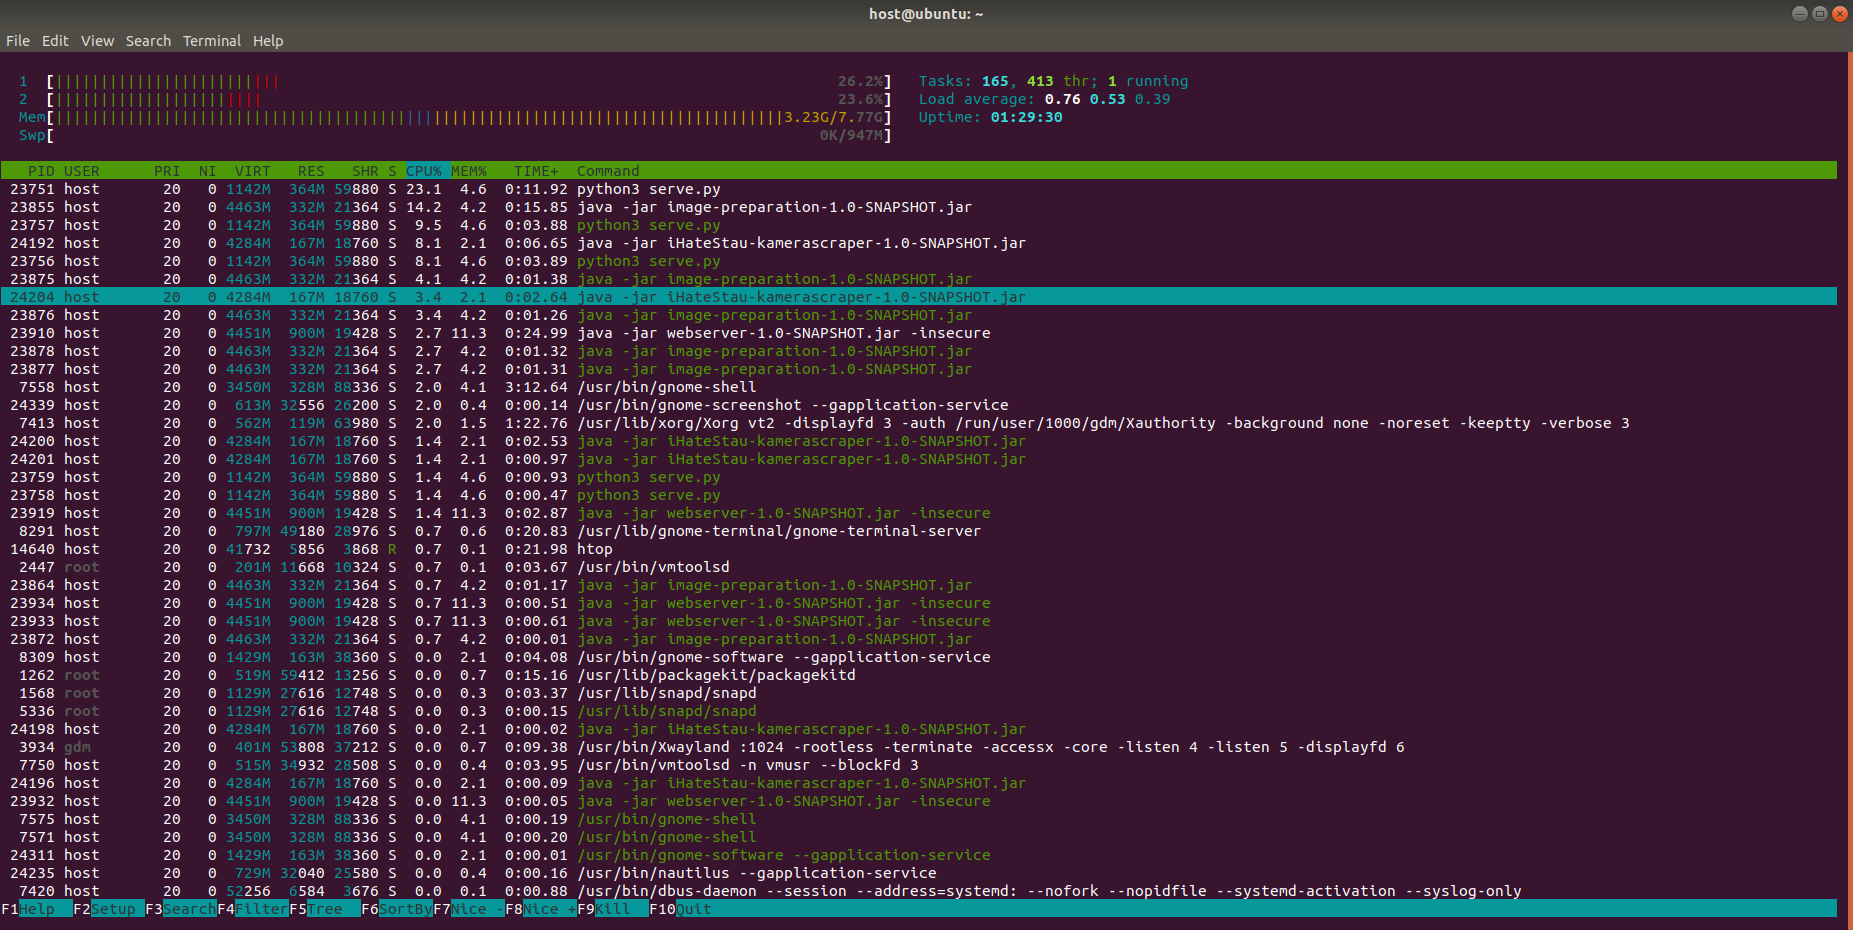
\includegraphics[width=15cm]{Bilder/server-ihatestau} \\
 \caption{Ressourcenverbrauch alter Server in htop}
 \label{fig:ihatestau-res}
\end{figure}
\begin{figure}[ht]
   \centering
     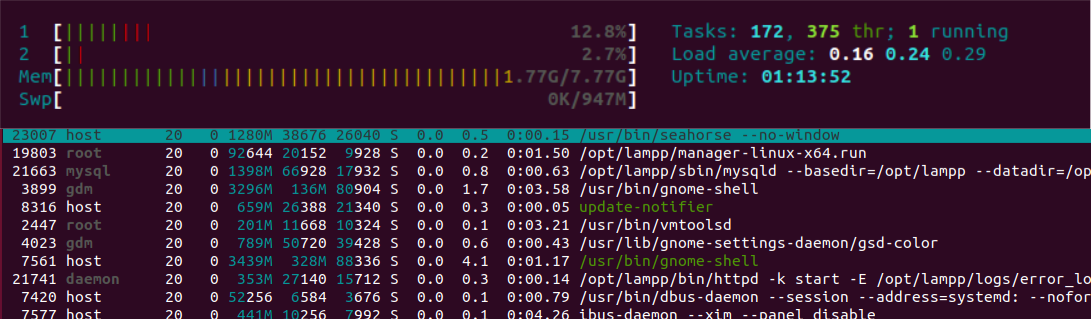
\includegraphics[width=15cm]{Bilder/server-new} \\
 \caption{Ressourcenverbrauch neuer Server in htop}
 \label{fig:new-server-res}
\end{figure}

Auf den Abbildungen~\ref{fig:ihatestau-res} und~\ref{fig:new-server-res} wird der Arbeitsspeicher- und CPU-Nutzungsbedarf des alten und neuen Backends visualisiert.

Bei dem Anblick der Abbildung wird auch klar, dass das alte System eher auf ein Anwendungsszenario im Großbetrieb ausgelegt war, da es sehr starken Gebrauch von Nebenläufigkeit und mehreren Threads macht.
Dies ist für ein Szenario in dem sehr viele Benutzer unterstützt werden sollen durchaus sinnvoll.
Jedoch bedeutet dies auch, dass das System einen hohen initialen Bedarf an Ressourcen hat, der sich pro Benutzer auch noch steigert.
In der Abbildung~\ref{fig:new-server-res} sieht man daher nur wenige Prozesse und keine Threads, die explizit von dem System verwendet werden.
Somit ist der Ressourcenverbrauch beim Starten des Systems stark reduziert.

Weiterhin werden auch weniger Ressourcen pro Benutzer benötigt.
Was hier jedoch ganz klar ein Nachteil im neuen System darstellt, ist, dass es nicht mehr für große Nutzermengen ausgelegt ist.
Es nutzt keine Skalierungsmaßnahmen wie Threads und Nebenläufigkeit aus und kann daher leicht bei großen Nutzerzahlen an die Systemgrenzen stoßen.

Diese Arbeit konzentriert sich auf den Betrieb des Backends für eine sehr kleine Nutzermenge, daher ist dieser Nachteil für das Ergebnis unerheblich.

\subsection{Frontend}
\begin{figure}[ht]
  \centering
	\begin{minipage}[b]{0.4\textwidth}
     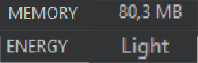
\includegraphics[width=\textwidth]{Bilder/res-app-old} \\
   \caption{Ressourcenverbrauch alter Client}
   \label{fig:res-app-old}
  \end{minipage}
	\hfill
	\begin{minipage}[b]{0.4\textwidth}
     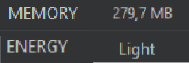
\includegraphics[width=\textwidth]{Bilder/res-app-new} \\
		\caption{Ressourcenverbrauch neuer Client}
		\label{fig:res-app-new}
	\end{minipage}
\end{figure}

Abbildung~\ref{fig:res-app-new} visualisiert einen Anstieg des Arbeitsspeicher-Verbrauchs im Vergleich zum alten Client, dessen Kennzahlen auf Abbildung~\ref{fig:res-app-old} zu sehen sind.
Dabei handelt es sich fast um eine Vervierfachung des ursprünglichen Arbeitsspeicherbedarfs.
Dies lässt sich natürlich vor allem durch die client-seitige Auswertung von Bildern erklären, da der hierfür benötigte Algorithmus mehrere Bilder im Arbeitsspeicher behält (siehe Abschnitt~\ref{sec:backsub-algo}).
Jedoch befindet sich der Arbeitsspeicherbedarf, selbst beim neuen Client, immer noch unter einem halben Gigabyte.

Mit den derzeitigen Hardware-Standards für Smartphones lässt sich dies gut vereinbaren, da aktuelle Smartphones bereits über mehrere Gigabytes an Arbeitsspeicher besitzen.
So lassen sich auch andere Applikationen parallel zur Verwendung des Clients nutzen.
Die Android Applikation "`YouTube"' benötigt beispielsweise ebenfalls etwa einen halben Gigabyte an Arbeitspeicher bei Benutzung.

Der Energiebedarf des neuen Clients ist laut dem Energy Profiler von Android Studio im Vergleich zum alten System gleich geblieben.
Dies lässt sich durch die wenigen Anfragen erklären, die der Client im Vergleich zum alten System tätigen muss.
Da der Client in einer Anfrage an das Backend direkt alle nötigten Bilder gesendet bekommt, muss er nicht einzeln anfragen.
Weiterhin verwendet der neue Client keine Google-APIs mehr, welche auch zusätzlichen Energiebedarf mit sich bringen.

Der gezeigte Wert für den Energieverbrauch ist jedoch nur gemittelt und als Rangmerkmal beschrieben, so kann es sein dass einzelne Ausreißer im Energieverbrauch der Applikation existieren. Um diese Ausreißer festzustellen, müsste jedoch eine konkrete Analyse der Applikation auf dem Betriebssystem des Smartphones stattfinden, welche im Rahmen dieser Arbeit übersprungen wurde.

\chapter{Zusammenfassung}

% Kritische, inhaltliche Reflexion von Theorie und Praxis 
\section{Fazit}
*Optimierter Algorithmus und optimierte Implementierung\newline
*Effizenz vs Genauigkeit\newline
*weniger dynamisch als mashine learning\newline
*

\section{Ausblick}
*Besseres Background-Model?\newline
*Mehr Vor-/Nach-Verarbeitung?\newline
*Genauere/Automatische Schwellwerte?\newline
*Alternative Datenquelle finden?\newline
*Mehr Features (Ausfahrten erkennung, Entfernung zur Ausfahrt)\newline
*Mehr UI-Features (Replay von Voice, Auswahl Kameras/Strecke)\newline


% ---------------------------- Literaturverzeichnis ----------------------------------------------
  \bibliographystyle{plainnat}
  \bibliography{Inhalt/literatur}

%\begin{thebibliography}{999999}


%\bibitem[FoBa03]{foobar2003} Foo, John; Bar, Belinda: \emph{Titel : Untertitel},\\ Verlagsort: Verlag, Jahr der Auflage. S. 10-20
%\bibitem[Le01]{levy2001} Autor Name: \emph{Titel des Buches}, New York: Penguin Books, 2001

%\end{thebibliography}

% ------------------------------- Anhang ---------------------------------------------------------

\appendix
\clearpage
\pagenumbering{Roman}						% römische Seitenzahlen für Anhang

%\includepdf[pages={1}]{Doc/TINF-Praxis-Bestaetigung.pdf}
%\includepdf[pages={1}]{Doc/TINF-Praxis-Reflexion.pdf}

\end{document}